% !Mode:: "TeX:UTF-8"
\chapter{基于一阶随机优化的编码衍射成像算法}
\label{chap:stochastic}
\section{引言}
当前,优化算法不断向着一阶、随机和非凸的趋势发展。一阶优化算法成为当今机器学习算法的主要原因是数据规模的不断增大。二阶或者更高阶算法由于需要计算或估计 Hessian 矩阵,这使得当问题规模很大时,数据的存储和读取往往困难或者难以实现。问题的规模庞大性也催化了随机算法的发展。在大规模情况下,数据的读取和存储代价高昂。随机算法正是为了克服这一缺点。在每次迭代中,随机地选取一部分样本用于梯度的计算,然后进进行随机梯度下降迭代。虽然随机梯度和目标函数在该次迭代的真实梯度有很大差距,但是在期望的角度,这种随机地选取往往都能够达到无偏统计以保证算法的收敛性。

非凸算法的发展则是由于近年来大量非凸问题的涌现,例如,深度学习问题往往都是非凸的。在工业应用中(如计算机视觉,人脸识别等),一阶随机非凸优化算取得了令人瞩目的成就。然而在传统的相位恢复的问题中,一阶随机非凸优化算法应用十分困难,主要原因在于相位恢复优化问题的耦合结构。为解决上述问题,Wu等人基于编码衍射模型中观测值可分离的特征提出了加速的On-RED(Online RED)算法。这是一阶随机优化算法首次应用于编码衍射成像领域。受到上述观点启发,本章提出了基于一阶随机优化的加速SOCE算法,如图\ref{fig:4-1}所示。
\begin{figure}[!hptb]
	\centering
	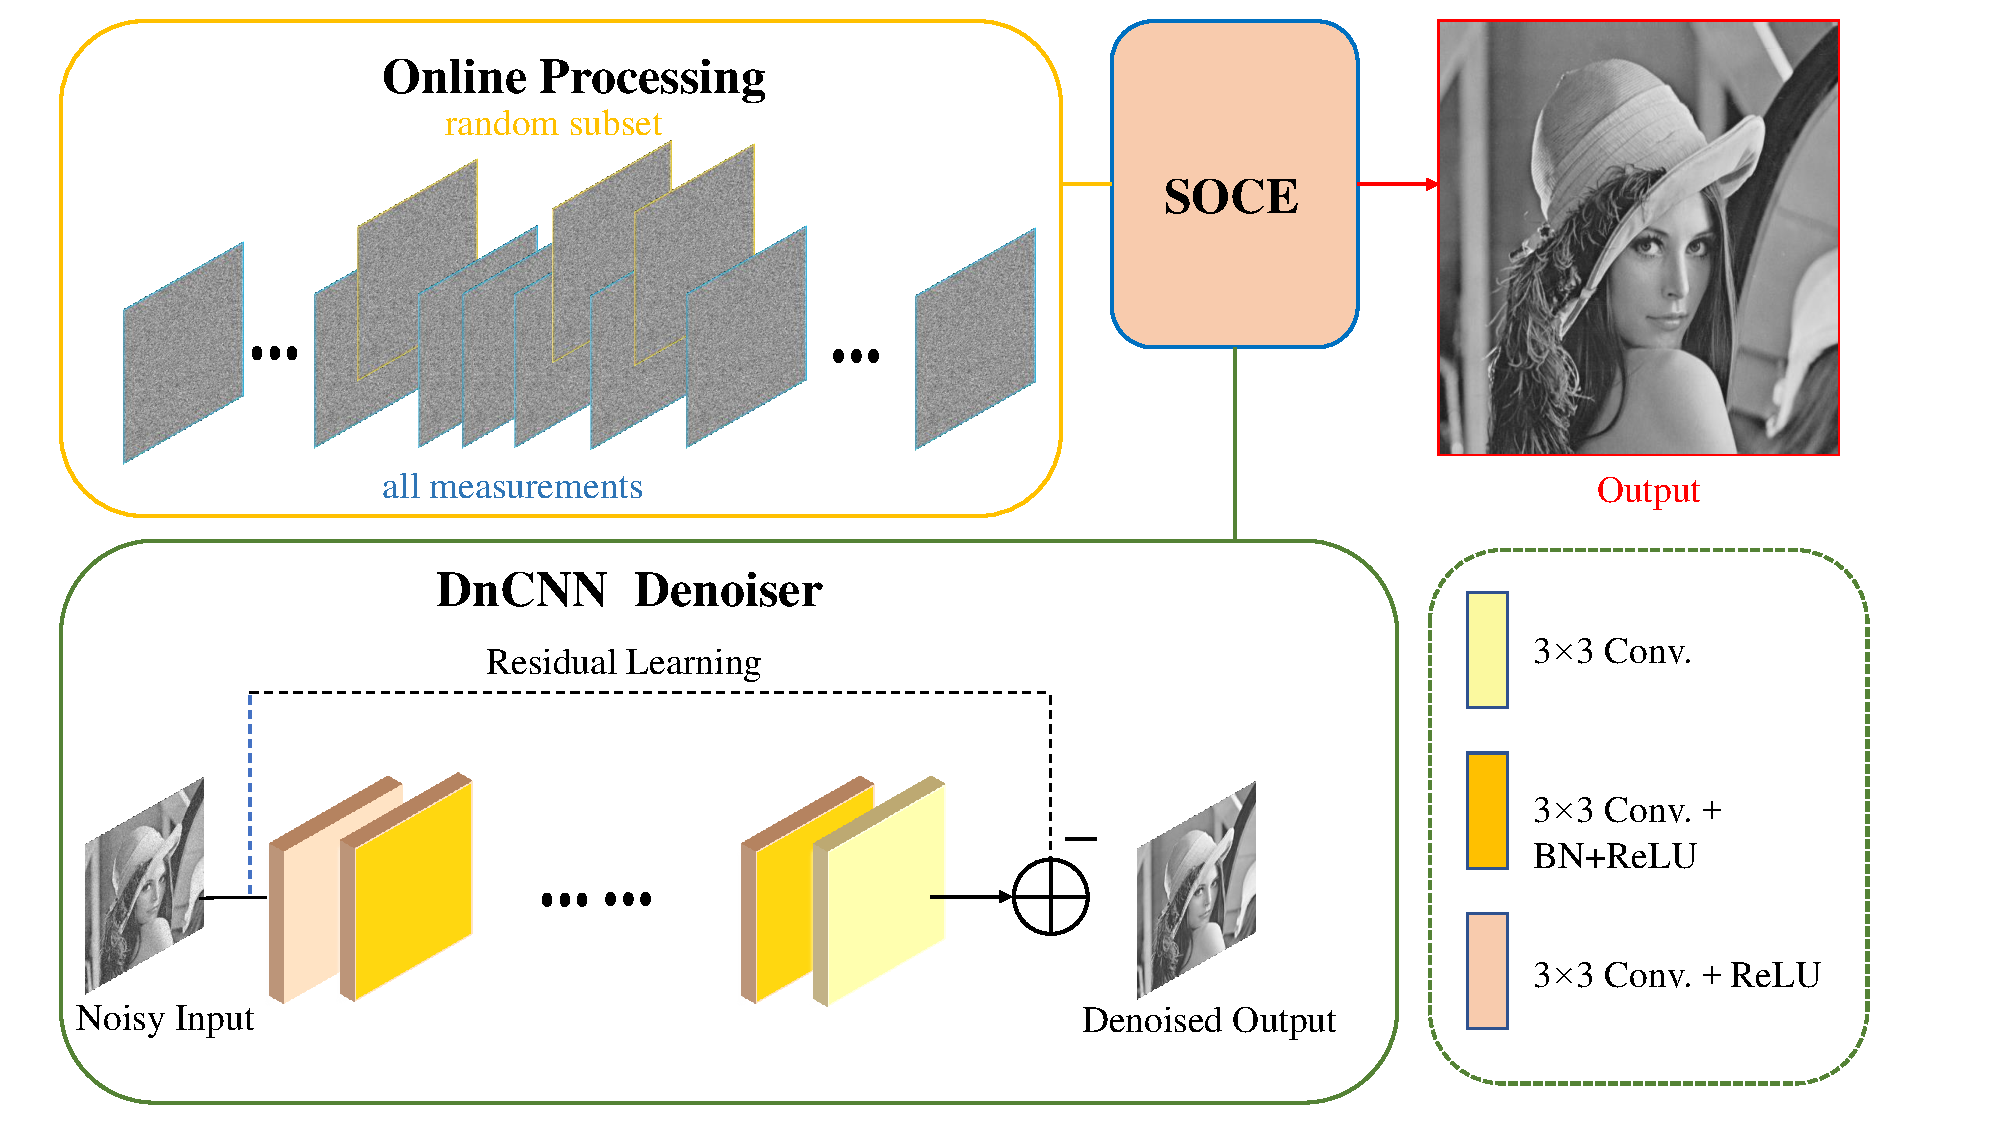
\includegraphics[height=0.5\linewidth, width=\linewidth]{4-1}
	\caption{SOCE算法结构示意图}\label{fig:4-1}
\end{figure}

\section{基于梯度的一阶随机优化算法}
经典的随机优化算法通常假设数据及代价函数各种属性的未知值(例如利普希茨常数、光滑性、强凸性常数或到最优点的距离)\supercite{Sun1,Sun2,Dongruo,Danilova,Chambolle2}。不幸的是,这些未知的属性值必须经过长时间的反复试验之后才能找到最优参数。为了有效解决这一问题,近年来许多无参数算法已经被开发用于在线优化和在线学习等任务。无参数算法对数据以及代价函数的性质不作任何假设,可能代价函数具体形式未知,但收敛速度与一般的最优化算法一样快。

在编码衍射成像中,基于即插即用的和RED先验的优化算法多数输入为为全部样本,算法每次迭代处理整个观测样本集合。对于大规模优化问题(数据集包含海量数据),基于随机优化的在线学习策略比整个样本集合处理的算法更加高效、灵活。%Metzler等人证实了使用DnCNN去噪器构造的RED先验在相位恢复中的取得SOTA(state-of-the-art)的结果,但是该算法在大规模编码衍射图案下运行速度较低。为了解决该问题,
鉴于此,Wu等人提出的On-RED算法的出现填补了随机优化在相位恢复领域的空白\supercite{Zihui}。On-RED算法的优化目标为问题\eqref{problem:3-4}。On-RED便是计算优化目标函数对输入数据集合的一个随机子集的梯度进行梯度下降,该算法在时间效率上优于一般的梯度下将算法\supercite{Zihui,Hong},并在目标函数为凸、去噪器为非扩张算子时,收敛速率为$O(\frac{1}{\sqrt{k}})$。编码衍射模型可用式子表示。对于优化目标问题\eqref{problem:3-4}的普通梯度下降算法为
\begin{equation} \label{method:4-1}
	x^{k+1}:=x^k-\eta(\nabla{f(x^k)}+\lambda{(x-D_{\sigma}(x^k))})
\end{equation}
其中$\eta>0$为迭代步长。现在对式\eqref{method:4-1}引入在线处理策略,这种机制受到数据保真项结构的限制。而编码衍射模型为多次可重复观测值,这决定了可对其随机子集进行梯度计算。对于数据保真项重新表示如下
\begin{equation} \label{method:4-2}
	f(x)=\mathbb{E}[f_i(x)]=\frac{1}{m}\sum_{i=1}^{m}f_i(x),
\end{equation}
其中$m$表示掩膜(mask)的数量,计算式\eqref{method:4-2}的梯度如下所示
\begin{equation} \label{equation:4-1}
	\nabla{f(x)}=\mathbb{E}[\nabla{f_i(x)}]=\frac{1}{m}\sum_{i=1}^{m}\nabla{f_i(x)},
\end{equation}
式\eqref{equation:4-1}正比于掩膜数量$m$。假设服从均匀随机分布的随机变量$i\in\{1,\ldots,m\}$,On-RED的关键在于每次迭代近似计算$B\ll{m}$个掩膜的平均梯度:
\begin{equation} \label{equation:4-2}
	\hat{\nabla}f(x)=\frac{1}{B}\sum_{b=1}^{B}\nabla{f_{i_{b}}(x)},
\end{equation}
其中$i_1,\ldots,i_B$为独立同分布于均匀分布的随机子集。小批样本数量$B\geq{1}$控制每次迭代计算近似梯度所需的样本数量。算法\ref{algorithm:4-1}总结了On-RED算法的实现细节,第二步采取深度学习中小批样本的方式计算随机选取的$B$个样本计算近似梯度。
\begin{algorithm}[!htbp]
	\setstretch{1.4}\zihao{-4}
	\caption{On-RED}
	\label{algorithm:4-1}
	\begin{algorithmic}[1]
		\REQUIRE	观测值$y\in \mathbb{R}^m$; % this command shows "Input"
		\ENSURE		% this command shows "Initialized"
		$\eta>0, \lambda>0, \sigma>0, B>0, x^0$随机; \\
		\WHILE {\emph{not converged}}
		\STATE	$\hat{\nabla}f(x)=\frac{1}{B}\sum_{b=1}^{B}\nabla{f_{i_{b}}(x)}$; \\  % line number at left side
		\STATE	$x^{k+1}=x^k-\eta{(\hat{\nabla}f(x) + \lambda(x^k-D_{\sigma}(x^k)))}$; \\	% line number at left side
		\ENDWHILE
		\RETURN 重构图像$x^{k+1}$.  % this command shows "Output"
	\end{algorithmic}
\end{algorithm}
\section{基于一阶随机优化的编码衍射成像算法}
受到On-RED算法的启发,本节将mini-batch随机计算梯度的方式应用于第三章提出的TACE算法数据保真项的近邻算子,提出了基于一阶随机优化的加速算法(SOCE)解决编码衍射成像中大规模编码衍射图案的相位恢复问题。SOCE的关键思想在于对数据保真项的近邻算子求解的随机化,其对应的优化问题为:
\begin{equation} \label{equation:4-3}
	\begin{aligned}
		\text{prox}_{\gamma{f}}(v)&=\arg\min_{x} \frac{1}{2}{\Vert{y-\vert{Ax}\vert}\Vert_2^2} + \frac{1}{2\gamma}{\Vert{x-v}\Vert_2^2},	\\
		&=\frac{1}{2m}\sum_{j=1}^{m}\big[y_{j}-\vert{a_{j}^\top x}\vert\big]^2+ \frac{1}{2\gamma}{\Vert{x-v}\Vert_2^2}.	\\
	\end{aligned}
\end{equation}
选取$B$个观测样本,应用mini-batch个样本计算上述优化问题的近似梯度,不动点$x^*$满足式\eqref{equation:4-4}:
\begin{equation} \label{equation:4-4}
	\frac{1}{B}\sum_{b=1}^{B}a_{j_b}^\mathit{T}\left({a_{j_b}^\top{x^*}-y\odot\frac{a_{j_b}^\top{x^*}}{\vert{a_{j_b}^\top{x^*}}\vert}}\right) + \frac{1}{\gamma}(x^*-v)=0,
\end{equation}
当$B=1$,优化问题\eqref{equation:4-3}可用随机不动点算法求解:
\begin{equation} \label{method:4-3}
	x^{k+1}:=\frac{1}{1+\gamma}\left(a_{j_b}^\mathit{T}\left({y\odot\frac{a_{j_b}^\top{x^k}}{\vert{a_{j_b}^\top{x^k}}\vert}}\right) + v\right).
\end{equation}
式\eqref{method:4-3}可推广至任意$B\ll{m}$,即如下所示:
\begin{equation} \label{method:4-4}
	x^{k+1}:=\frac{1}{1+\gamma}\left(\frac{1}{B}\sum_{b=1}^{B}a_{j_b}^\mathit{T}\left({y\odot\frac{a_{j_b}^\top{x^k}}{\vert{a_{j_b}^\top{x^k}}\vert}}\right) + v\right).
\end{equation}
其中$j_1,\ldots,j_B$为独立同分布于$\{1,\ldots,m\}$之上的均匀分布的子集。此时式\eqref{method:4-4}不再与$prox_{\gamma{f}}(v)$严格相等。所以将式\eqref{method:4-4}记作$prox_{\gamma{\hat{f}}}(v)$。为了与TACE算法的式\eqref{equation:agent}有所区别,于是令$\mathbf{\hat{F}}(\mathbf{v})=(prox_{\gamma{\hat{f}}}(v_1),D_{\sigma}(v_2))^\top$。相应地,定义$\hat{T}=(2G_{\mu}-I)(2\hat{F}-I)$。算法\ref{algorithm:4-2}总结了SOCE算法的实现细节。
\begin{algorithm}[!htbp]
	\setstretch{1.4}\zihao{-4}
	\caption{SOCE}
	\label{algorithm:4-2}
	\begin{algorithmic}[1]
		\REQUIRE	观测值$y\in \mathbb{R}^m$; % this command shows "Input"
		\ENSURE		% this command shows "Initialized"
		$\alpha,\beta\in(0,1),\gamma{=1},sigma\in[1,50],B>0,(\mathbf{v}^0,x^0)$随机; \\
		\WHILE {\emph{not converged}}
		\STATE	$\mathbf{v}^{k+1}:=(1-\beta)\mathbf{v}^{k}+\beta\hat{\mathbf{T}}(\mathbf{v}^{k})$;	\\  % line number at left side
		\STATE	$x^{k+1}:=(1-\alpha)x^k + \alpha\overline{\mathbf{v}}^{k+1}$; \\	% line number at left side
		\ENDWHILE
		\RETURN 重构图像$x^{k+1}$. % this command shows "Output"
	\end{algorithmic}
\end{algorithm}

\section{实验结果及分析}
本章所提的SOCE算法采用与第三章相同的内部参数设置,并将$B=1$作为SOCE算法的mini-batch。对比算法为固定一个(fix 1)与四个(fix 4)随机掩膜的TACE算法。由于On-RED算法为numpy实现,其运行在CPU上,而SOCE运行在GPU上,故暂不做为对比选项。实验仿真平台为:Intel(R) Xeon(R) CPU E5-2650 v4处理器(2.20GHz),252G内存,ubuntu 16.04操作系统, Tesla K80显卡,cuda 10.2,cudnn 7605。

\subsection{抗高斯噪声模型}
本节给出了观测值高斯噪声占比SNR=15dB时SOCE算法的图像质量评价指标(PSNR/SSIM)与平均运行时间(Averaged Run-Time)。注意去噪算子对比顺序为DnCNN/IRCNN。SOCE算法的PSNR、SSIM、平均运行时间如表\ref{table:4-1}所示。
\begin{table}[!htbp]
	\def\arraystretch{1.4}\centering\zihao{5}
	\caption{不同mini-batch不同去噪器下获得平均PSNR(dB)/SSIM/Run-Time(s)比较}
	\label{table:4-1}
	\begin{tabular*}{\linewidth}{@{}@{\extracolsep{\fill}}cccc@{}}
		\toprule
		mini-batch	& fixed 1 & B=1 & fixed 4\\ %\cmidrule(r){2-4}
		\midrule
		Avg PSNR        & 30.82/30.63   & 33.34/33.06  & {\color{red}34.31}/{\color{red}33.93} \\
		Avg SSIM        & 0.8209/0.8319   & 0.8584/0.8659  & {\color{red}0.9005}/{\color{red}0.9035} \\
		Avg Run-Time    & {\color{blue}30.68}/12.03   & 49.93/15.95  & 30.81/{\color{blue}11.62} \\
		\bottomrule
	\end{tabular*}
\end{table}

表\ref{table:4-1}表明,在高斯噪声强度占比SNR=15dB下,SOCE算法当mibi-batch为$B=1$时,其PSNR比单个固定的TACE算法高2.54dB,但比四个观测值得TACE算法低0.97dB。从两者的差值可以看出SOCE算法对高斯噪声的泛化能力,这得益于SOCE算法每次迭代随机从衍射图案集合抽取$B$个元素的子集。但是平均运行时间却出乎预料:SOCE算法的运行时间高于四个衍射图案的TACE算法。其原因在于SOCE算法随机选取衍射图案使用CPU消耗一定的时间并且本实验仅有四个掩膜,未达到百万量级,SOCE算法的加速性能无法体现。限于计算资源的有限,这个疑问作为以后研究验证。

为了从主观视觉上比较SOCE算法重构效果,本节给出了不同mini-batch下重构Barbara与Pollen图像的自对比结果,如图\ref{fig:4-2}、图\ref{fig:4-3}所示。
\begin{figure}[!htbp]
	\centering
	\subfigure[Original]{
		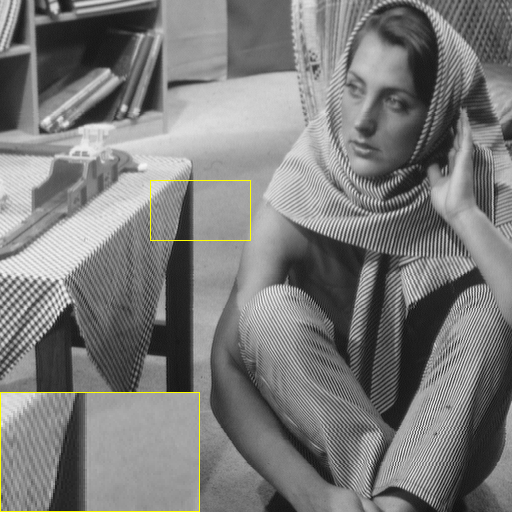
\includegraphics[width=0.2\linewidth]{4-2-1}
	}\hspace{-0.01\linewidth}
	\subfigure[fix 1/27.61]{
		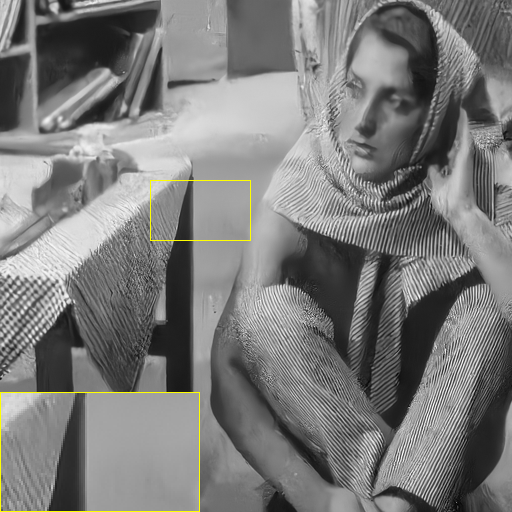
\includegraphics[width=0.2\linewidth]{4-2-3}
	}\hspace{-0.01\linewidth}
	\subfigure[B=1/30.64]{
		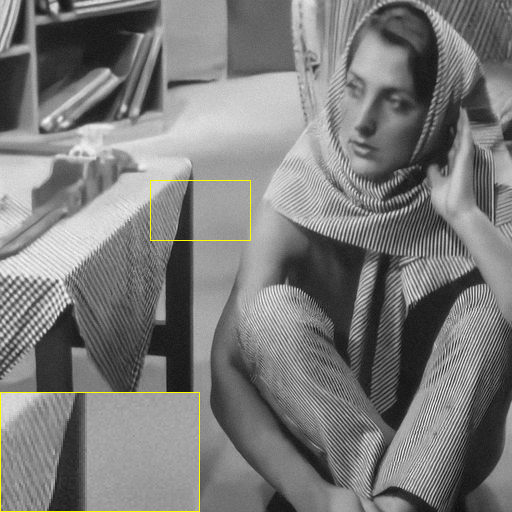
\includegraphics[width=0.2\linewidth]{4-2-5}
	}\hspace{-0.01\linewidth}
	\subfigure[fix 4/{\color{red}34.31}]{
		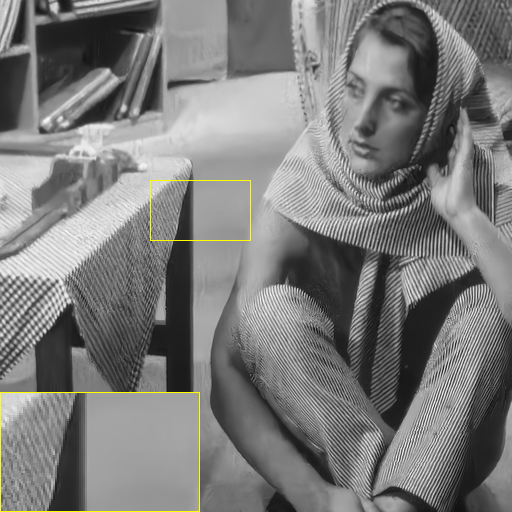
\includegraphics[width=0.2\linewidth]{4-2-7}
	}
	
	\subfigure[Original]{
		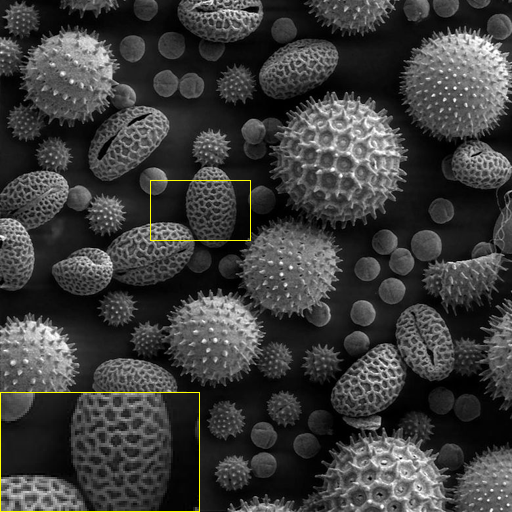
\includegraphics[width=0.2\linewidth]{4-2-2}
	}\hspace{-0.01\linewidth}
	\subfigure[fix 1/28.44]{
		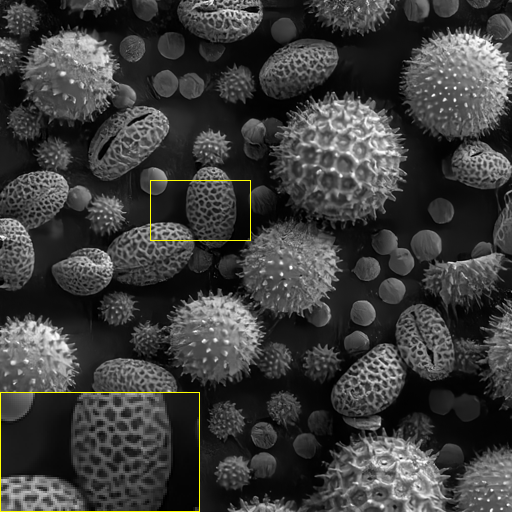
\includegraphics[width=0.2\linewidth]{4-2-4}
	}\hspace{-0.01\linewidth}
	\subfigure[B=1/32.50]{
		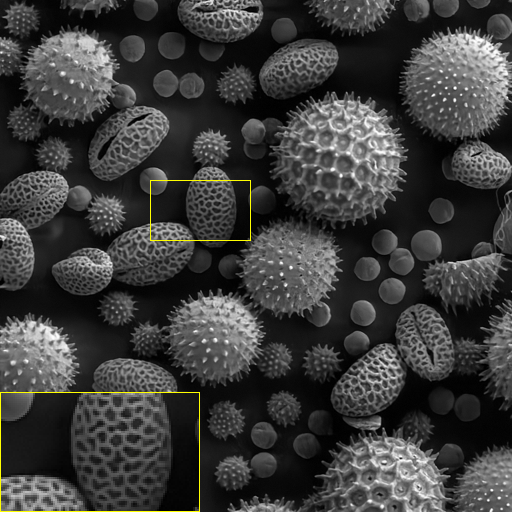
\includegraphics[width=0.2\linewidth]{4-2-6}
	}\hspace{-0.01\linewidth}
	\subfigure[fix 4/{\color{red}32.92}]{
		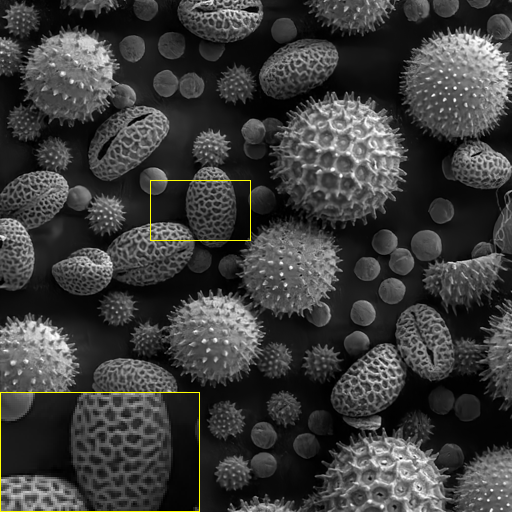
\includegraphics[width=0.2\linewidth]{4-2-8}
	}
	\caption{SOCE算法在DnCNN下不同mini-batch的重构结果} 
	\label{fig:4-2} 
\end{figure}
\begin{figure}[!htbp]
	\centering
	\subfigure[Original]{
		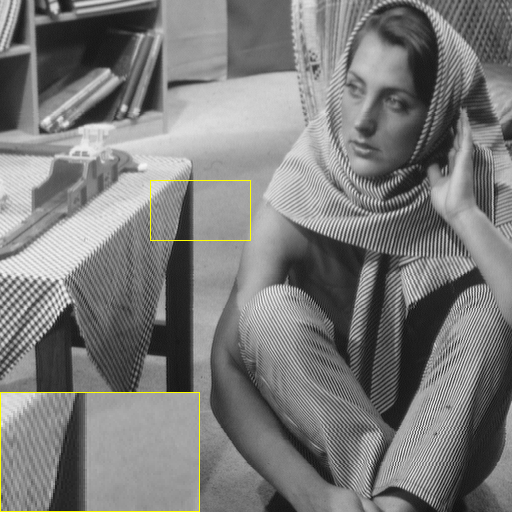
\includegraphics[width=0.2\linewidth]{4-3-1}
	}\hspace{-0.01\linewidth}
	\subfigure[fix 1/27.26]{
		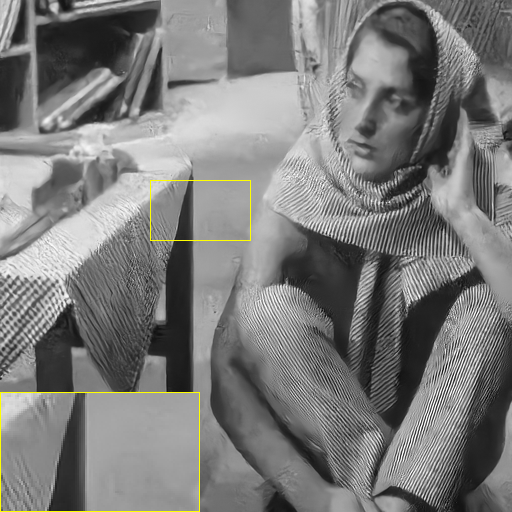
\includegraphics[width=0.2\linewidth]{4-3-3}
	}\hspace{-0.01\linewidth}
	\subfigure[B=1/29.87]{
		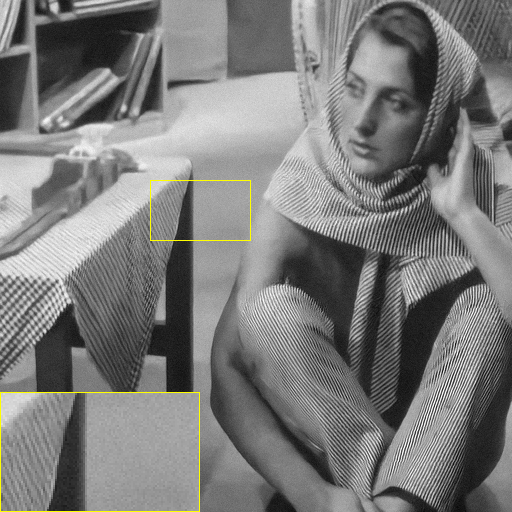
\includegraphics[width=0.2\linewidth]{4-3-5}
	}\hspace{-0.01\linewidth}
	\subfigure[fix 4/{\color{red}32.58}]{
		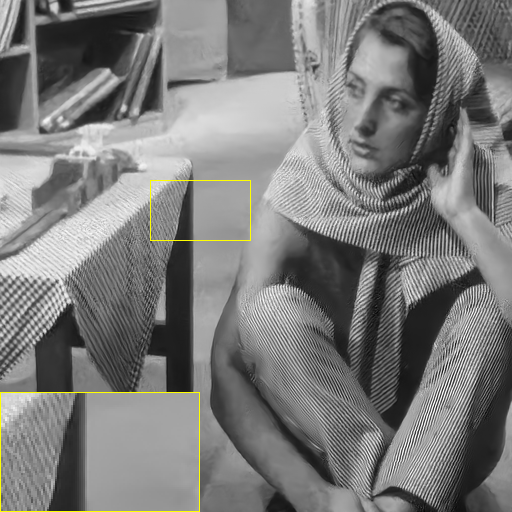
\includegraphics[width=0.2\linewidth]{4-3-7}
	}
	
	\subfigure[Original]{
		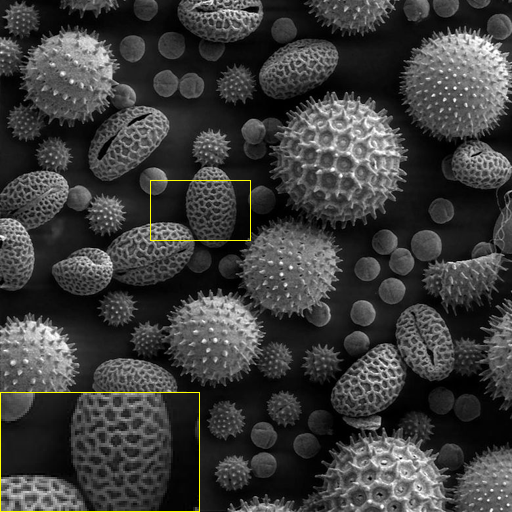
\includegraphics[width=0.2\linewidth]{4-3-2}
	}\hspace{-0.01\linewidth}
	\subfigure[fix 1/28.34]{
		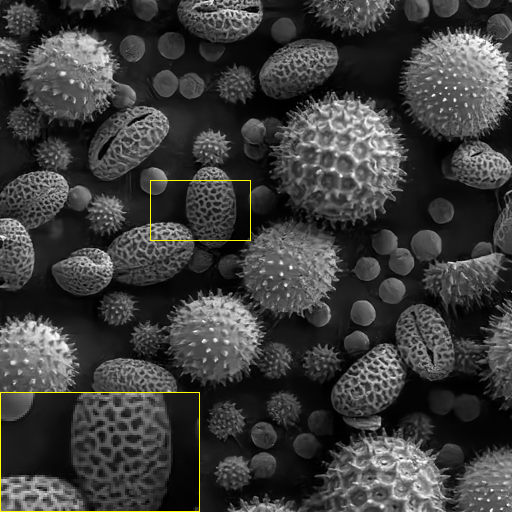
\includegraphics[width=0.2\linewidth]{4-3-4}
	}\hspace{-0.01\linewidth}
	\subfigure[B=1/{\color{red}32.34}]{
		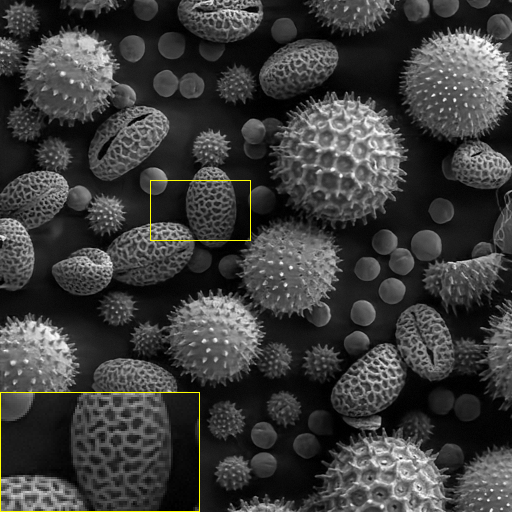
\includegraphics[width=0.2\linewidth]{4-3-6}
	}\hspace{-0.01\linewidth}
	\subfigure[fix 4/30.60]{
		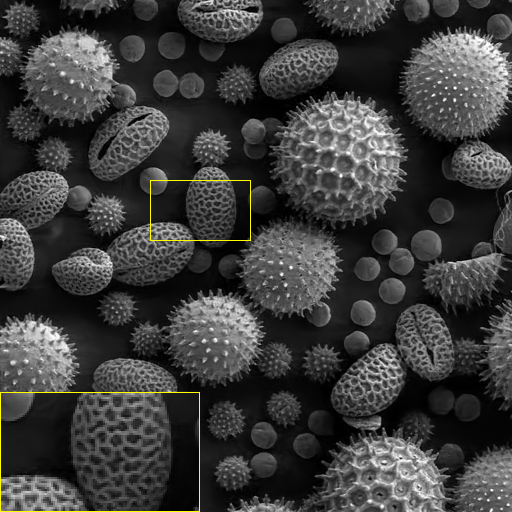
\includegraphics[width=0.2\linewidth]{4-3-8}
	}
	\caption{SOCE算法在IRCNN下不同mini-batch的重构结果}
	\label{fig:4-3}
\end{figure}

从图\ref{fig:4-2}与图\ref{fig:4-3}可以看出,SOCE算法重构图像质量优于单个固定掩膜的TACE算法,其重构图像的细节、纹理等信息更加丰富。

因SOCE算法引入了随机性,在特定假设下证明该算法的收敛性困难较大,故定性地利用数据保真项的近邻算子与DnCNN去噪算子在算法迭代过程中的局部利普希茨常数统计直方图来验证SOCE算法的收敛性,重构Barbara迭代过程中利普希茨常数的统计直方图如图\ref{fig:4-4}所示。图\ref{fig:4-4}中的\subref{subfigure:4-1-1}为单个衍射图案时TACE算法数据保真项近邻算子与去噪器在迭代过程中的利普希茨常数统计直方图,\subref{subfigure:4-1-2}为$B=1$时SOCE算法数据保真项近邻算子与去噪器在迭代过程中的利普希茨常数统计直方图,\subref{subfigure:4-1-3}为四个衍射图案时TACE算法数据保真项近邻算子与去噪器在迭代过程中的利普希茨常数统计直方图。上层代表数据保真项的近邻算子,下层代表DnCNN去噪算子。从中可以看出,利普希茨常数统计直方图近似服从高斯分布,故SOCE算法对噪声更具泛化性。
\begin{figure}[!htbp]
	\centering
	\subfigure[fix 1]{
		\label{subfigure:4-1-1}
		\begin{minipage}[t]{0.2\linewidth}
			\centering
			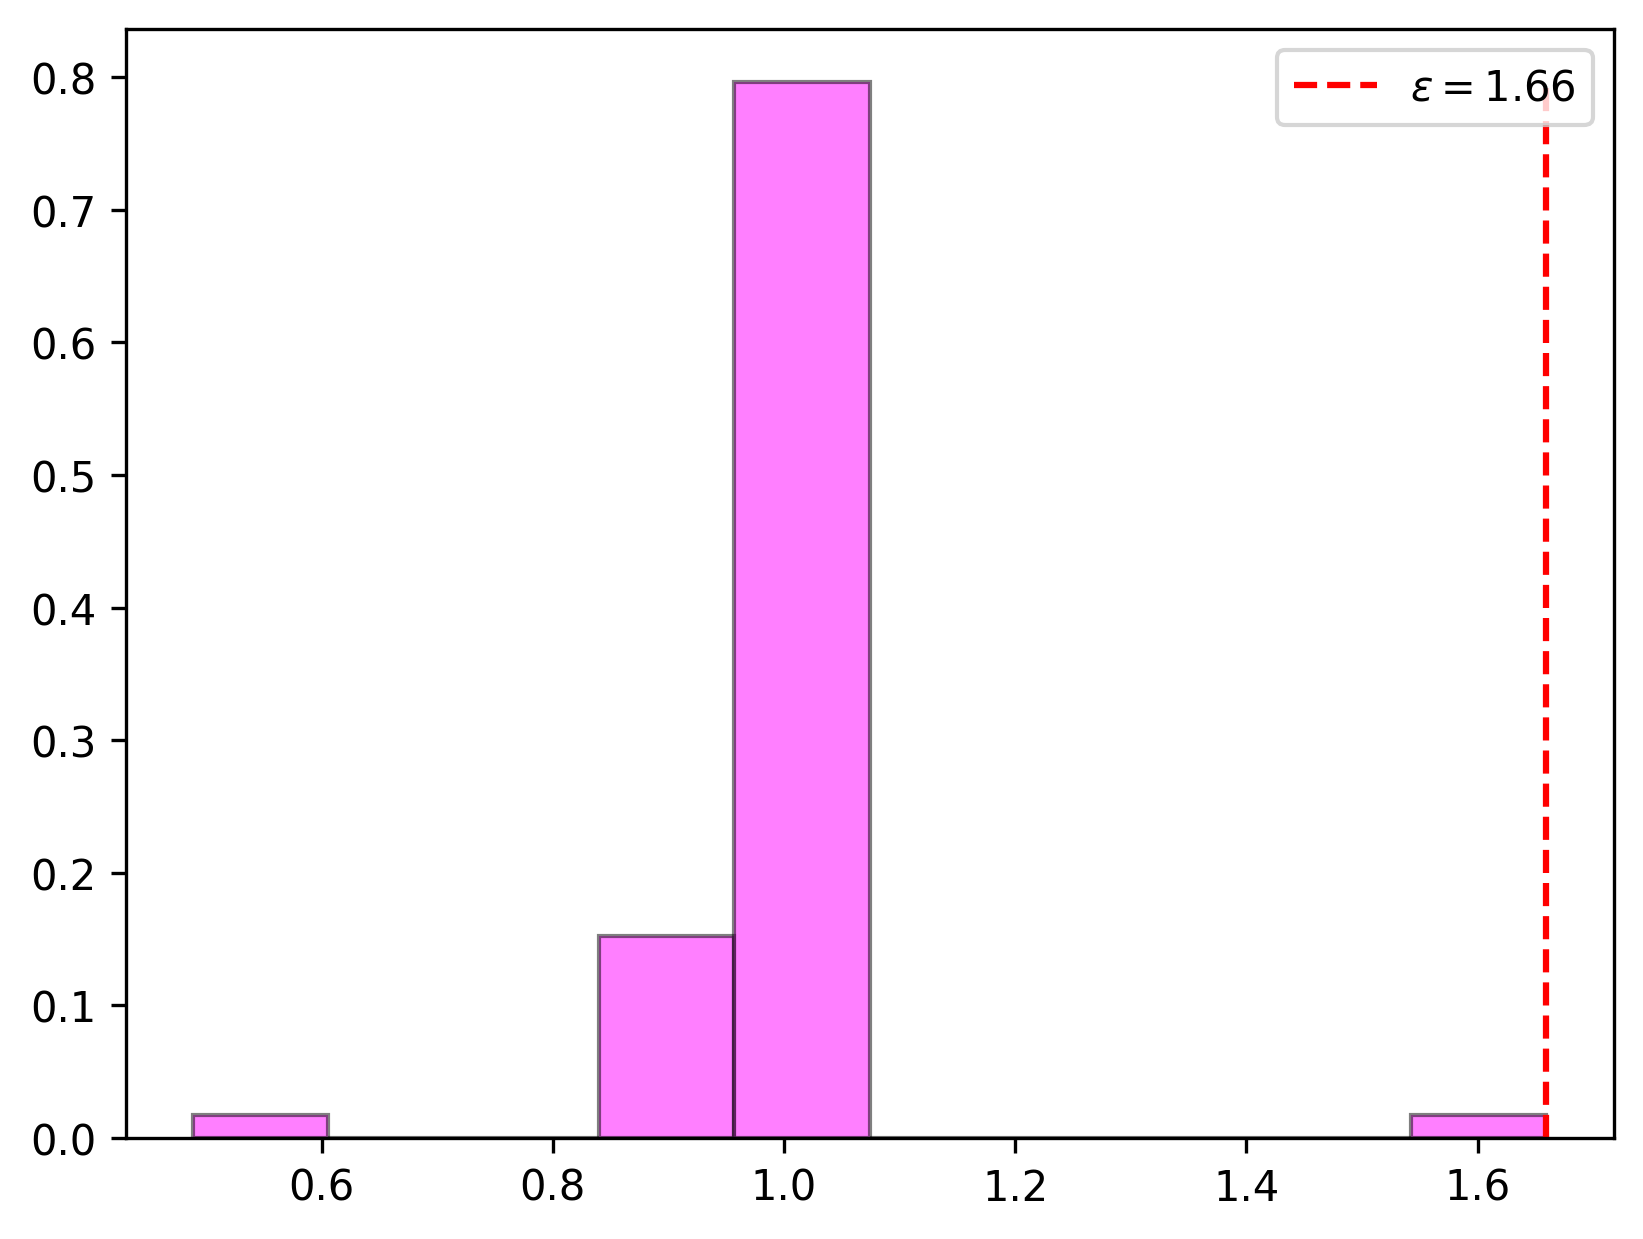
\includegraphics[width=\linewidth]{4-4-1}\\
			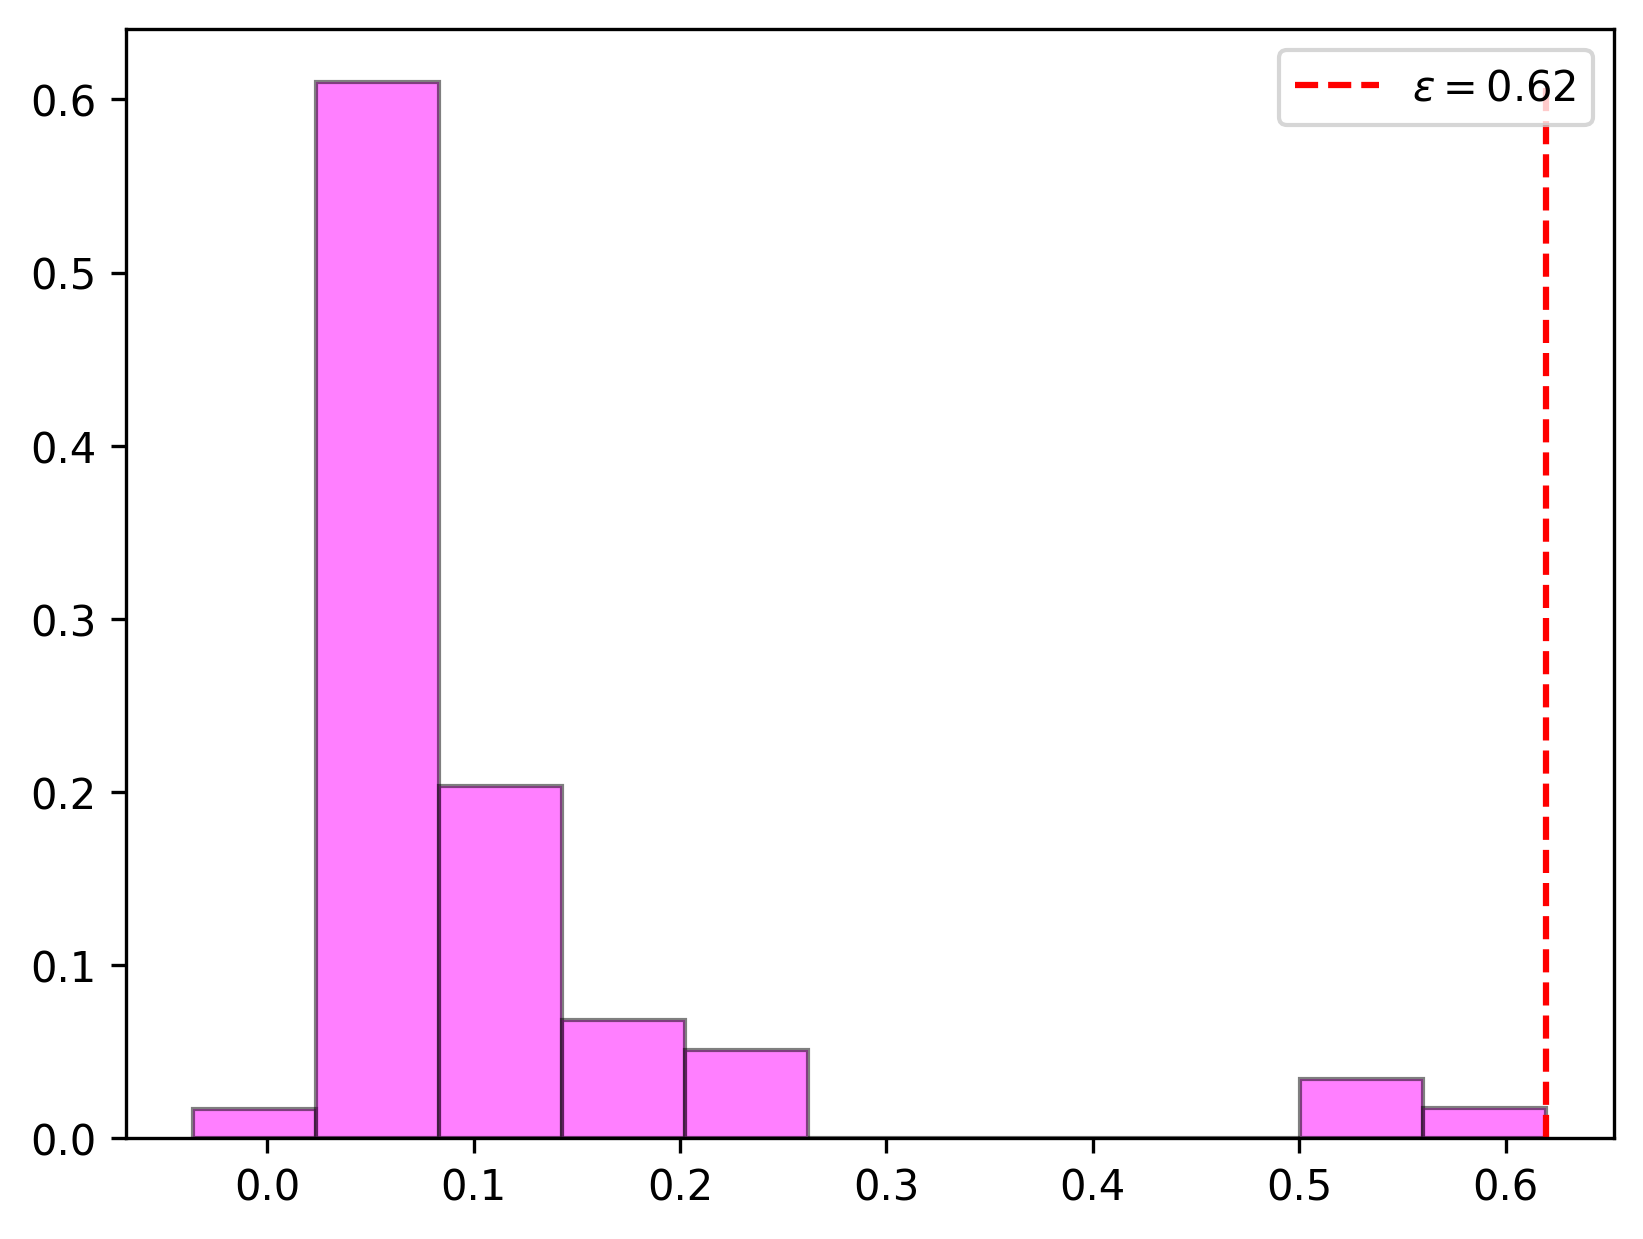
\includegraphics[width=\linewidth]{4-4-2}
			%\caption{fig}
		\end{minipage}
	}
	\subfigure[B=1]{
		\label{subfigure:4-1-2}
		\begin{minipage}[t]{0.2\linewidth}
			\centering
			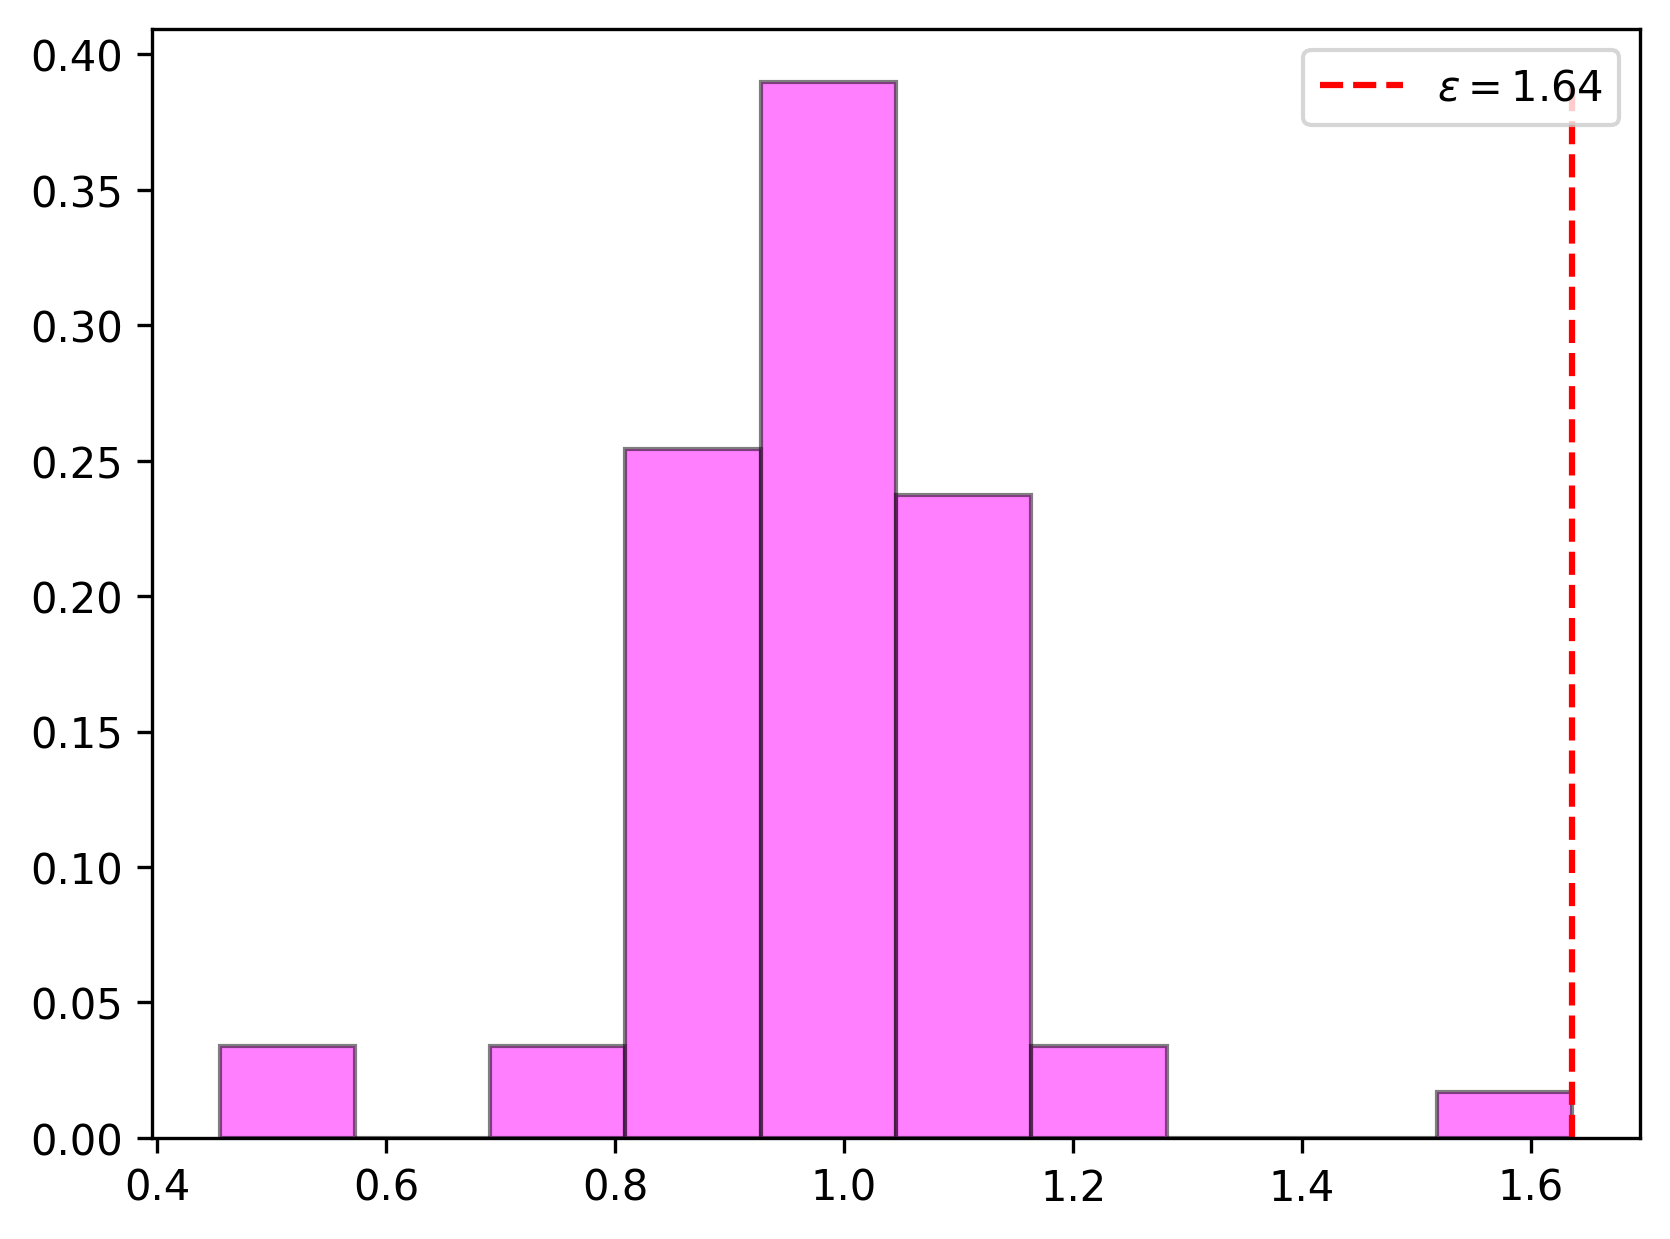
\includegraphics[width=\linewidth]{4-4-3}\\
			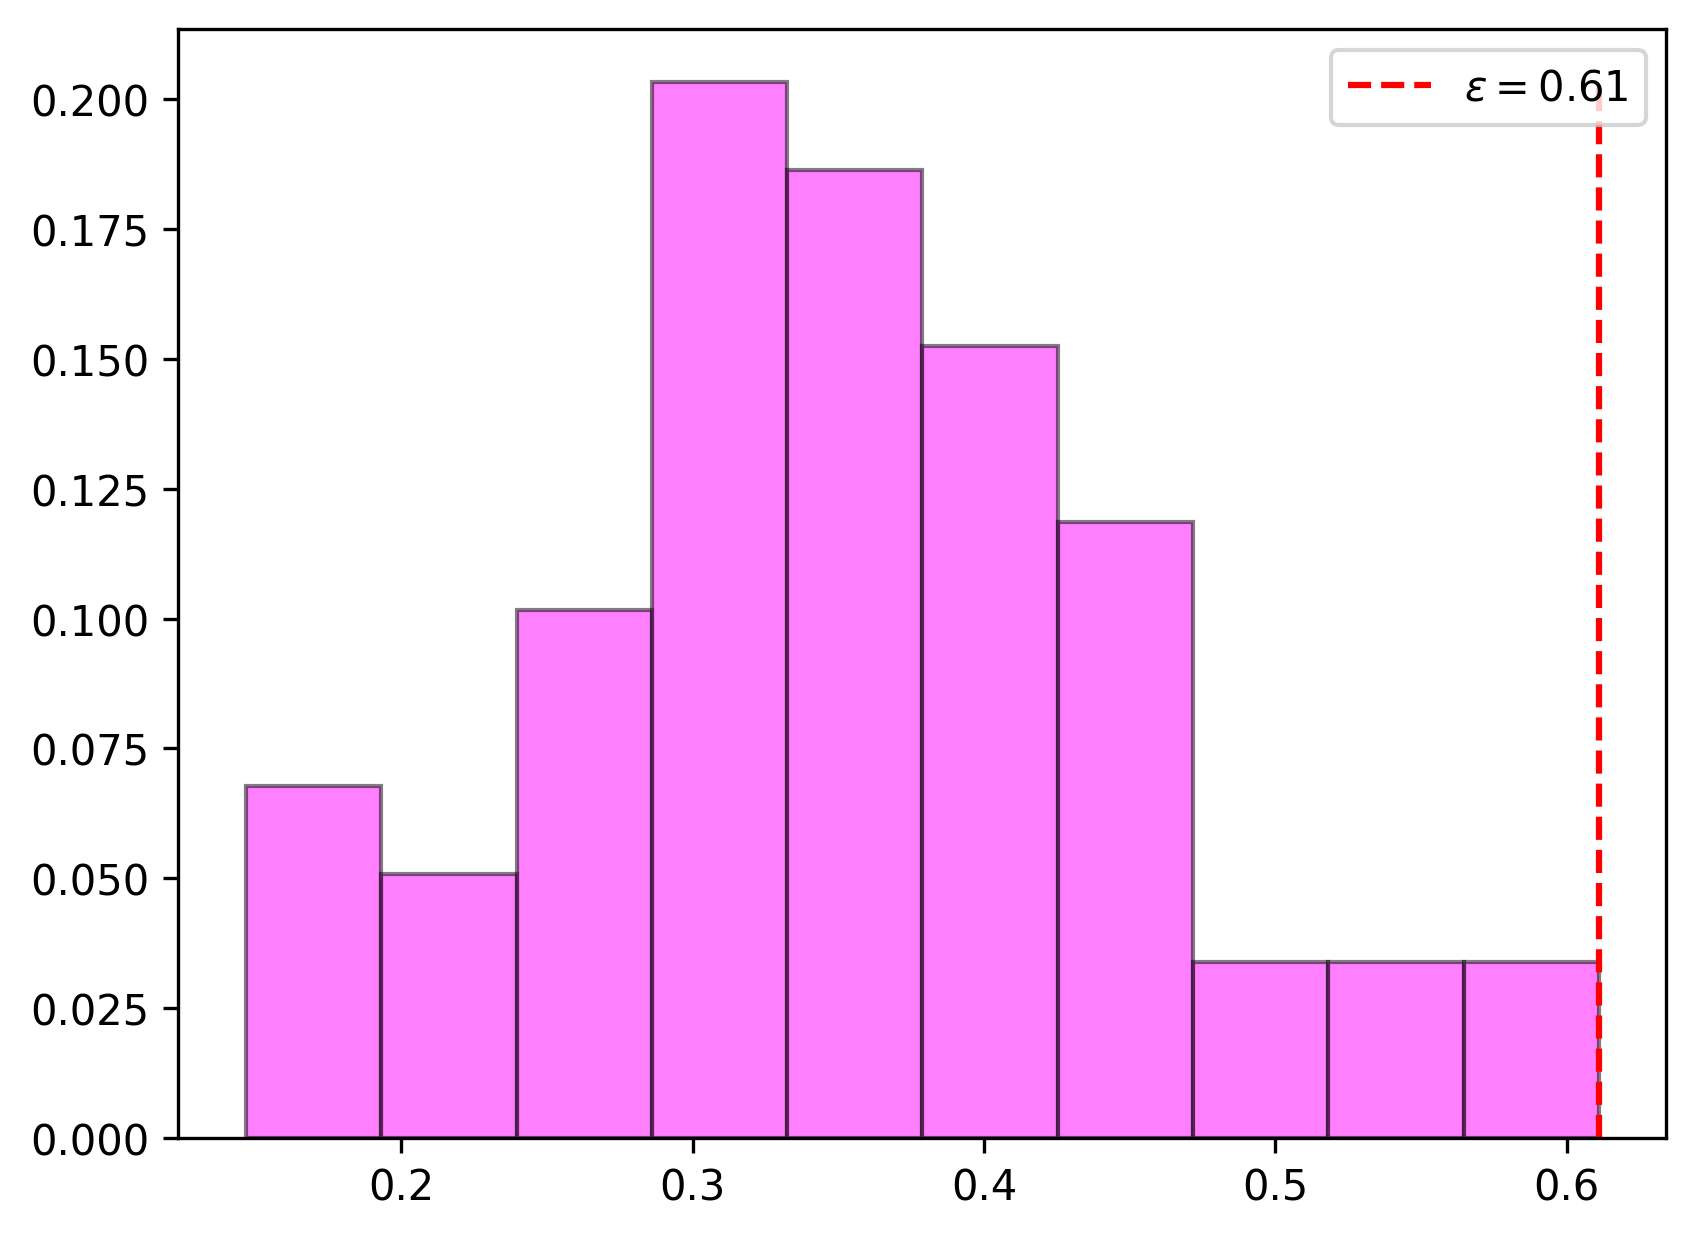
\includegraphics[width=\linewidth]{4-4-4}
			%\caption{fig}
		\end{minipage}
	}
	\subfigure[fix 4]{
		\label{subfigure:4-1-3}
		\begin{minipage}[t]{0.2\linewidth}
			\centering
			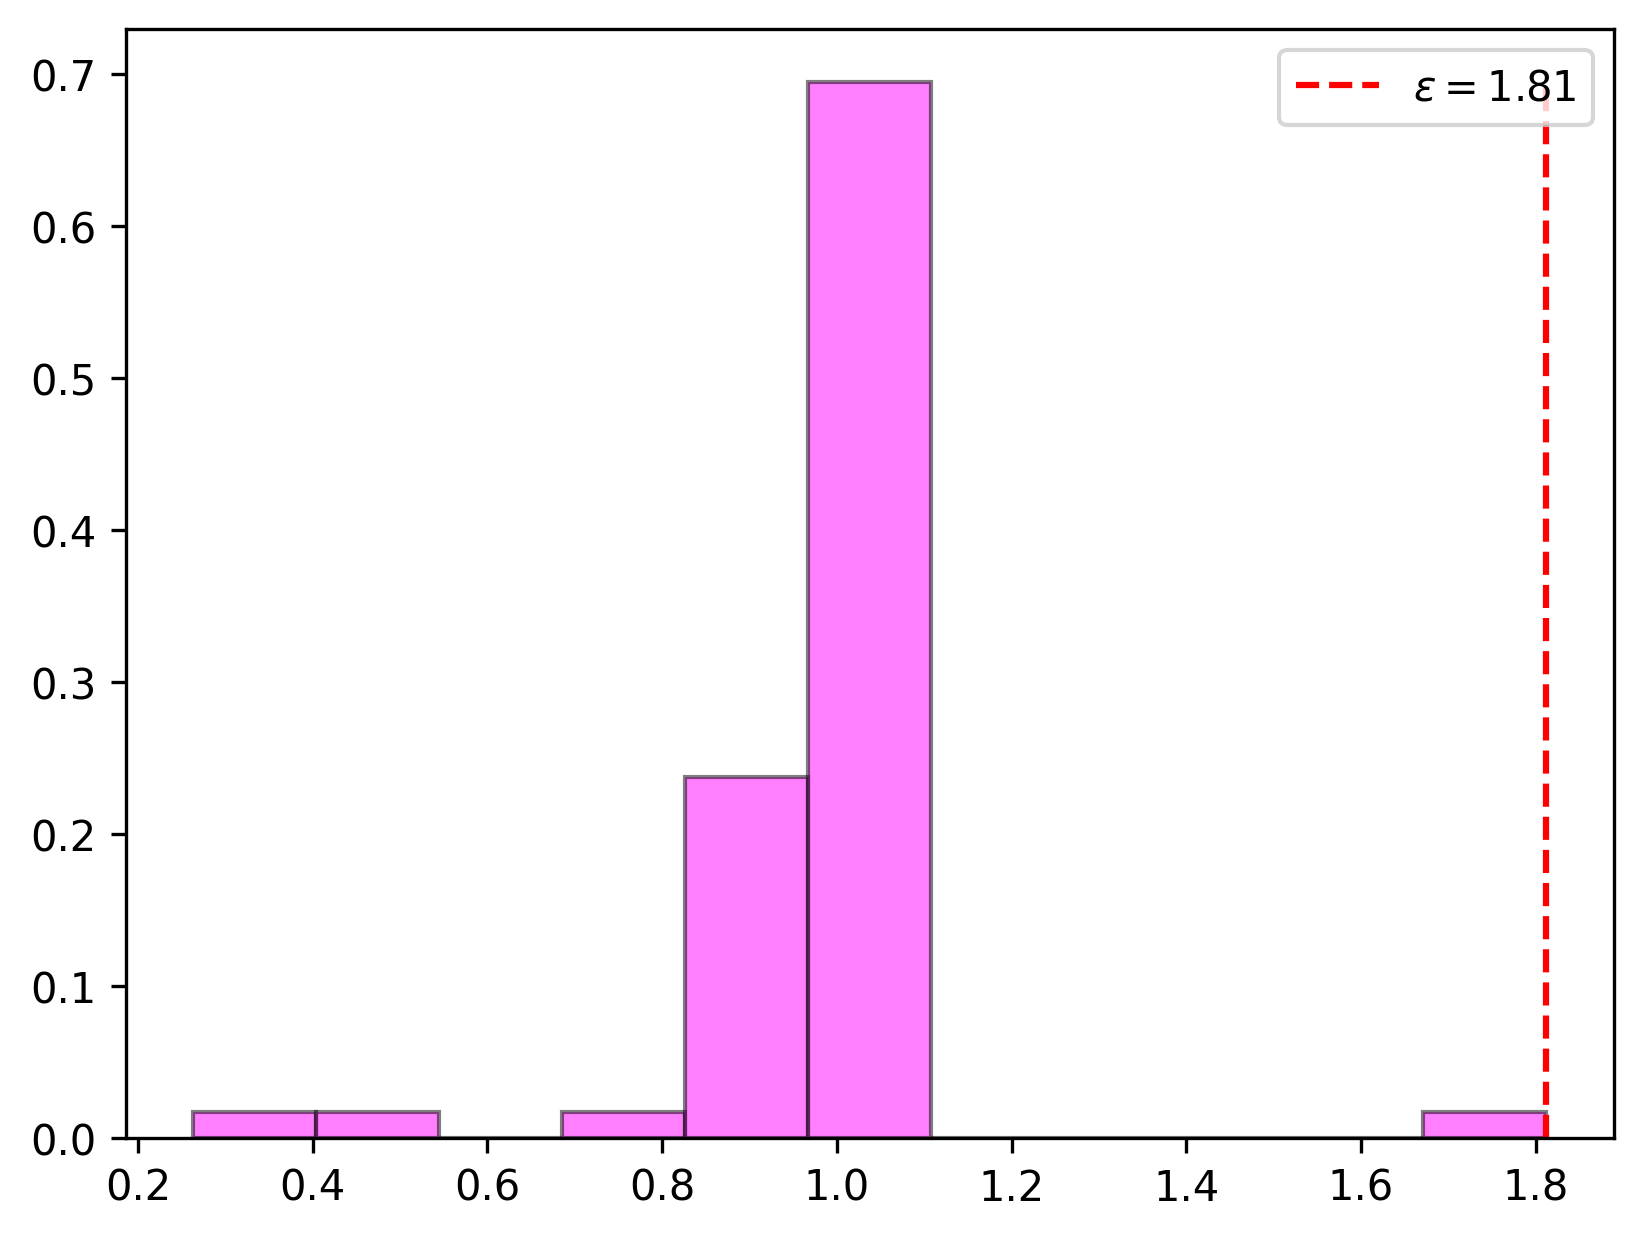
\includegraphics[width=\linewidth]{4-4-5}\\
			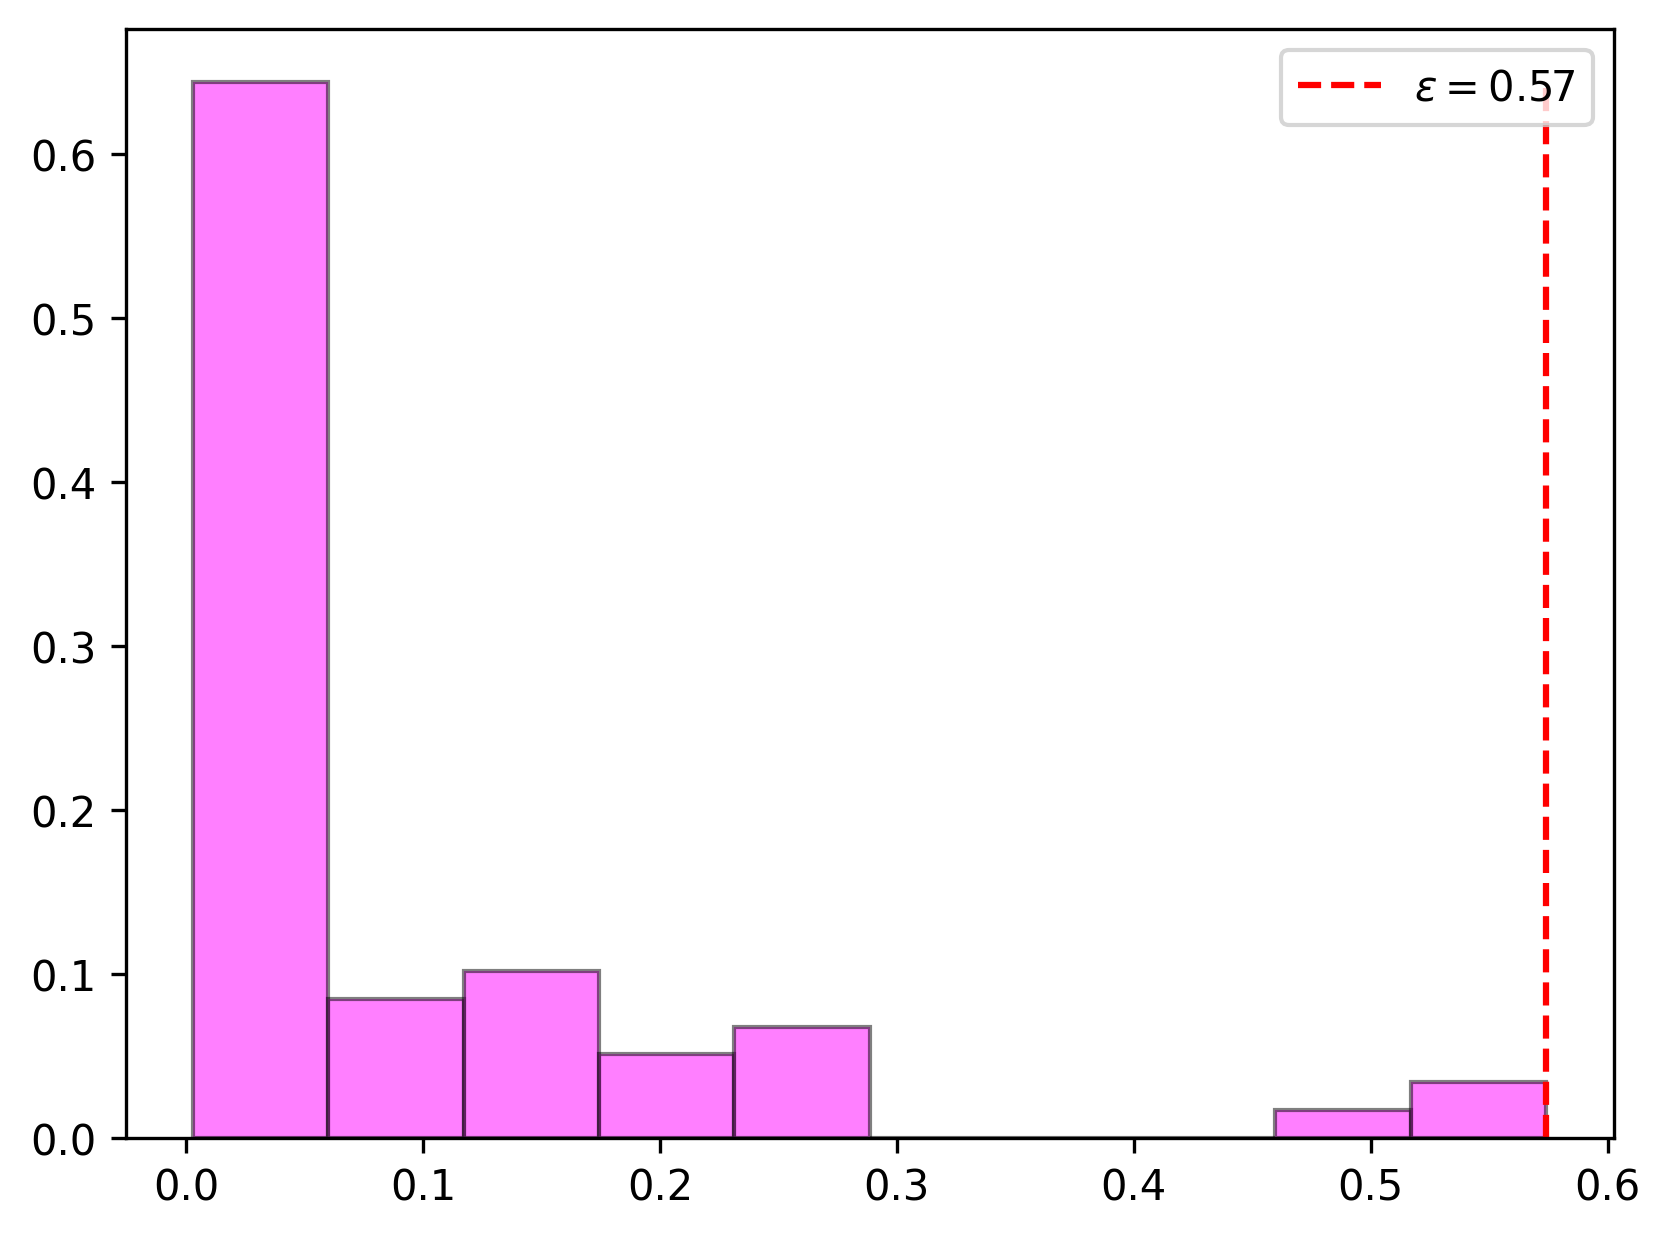
\includegraphics[width=\linewidth]{4-4-6}
			%\caption{fig}
		\end{minipage}
	}
	\caption{SOCE算法在迭代过程中的利普希茨常数统计直方图(DnCNN)} 
	\label{fig:4-4}
\end{figure}

\subsection{抗泊松噪声模型}
本节给出了泊松噪声强度$\alpha=81$时SOCE算法重构图像的评价指标与平均运行时间。SOCE算法的PSNR、SSIM、平均运行时间如表\ref{table:4-2}所示。
\begin{table}[!htbp]
	\def\arraystretch{1.4}\centering\zihao{5}
	\caption{不同mini-batch在不同去噪器下获得平均PSNR(dB)/SSIM/Run-Time(s) 比较}
	\label{table:4-2}
	\begin{tabular*}{\linewidth}{@{}@{\extracolsep{\fill}}cccc@{}}
		\toprule
		mini-batch	& fixed 1 & B=1 & fixed 4\\ %\cmidrule(r){2-4}
		\midrule
		Avg PSNR        & 25.56/25.56   & 27.10/27.18  & {\color{red}28.29}/{\color{red}28.32} \\
		Avg SSIM        & 0.6835/0.6862   & 0.6702/0.6935  & {\color{red}0.8073}/{\color{red}0.8220} \\
		Avg Run-Time    & {\color{blue}33.74}/{\color{blue}12.17}   & 44.15/14.06  &46.88/12.85 \\
		\bottomrule
	\end{tabular*}
\end{table}

表\ref{table:4-2}表明:在泊松噪声强度$\alpha=81$、不同去噪器下,SOCE算法当mibi-batch为$B=1$时,其平均PSNR比单个固定的TACE算法高1.54dB/1.62dB,但比四个观测值得TACE算法低1.19dB/1.14dB;SOCE算法的平均SSIM比单个固定的TACE算法高-0.0133/0.0073,但比四个观测值得TACE算法低0.1371/0.1285。值得注意的是SSIM在DnCNN去噪算子下SOCE算法出现了反例。不过从两者其他的差值可以看出同上节抗高斯噪声的结论相同,平均运行时间的结论亦相同。

为了从主观视觉上比较SOCE算法重构效果,本节展示了不同mini-batch下重构Barbara与Pollen图像的自对比结果,如图\ref{fig:4-5}、图\ref{fig:4-6}所示。从图\ref{fig:4-5}与图\ref{fig:4-6}的黄色框中的放大细节可以明显看出,SOCE算法重构的纹理与细节多于单个衍射图案的TACE算法。但与使用四个掩膜的TACE算法相差1.19dB,这表明SOCE算法仍有改进的潜力。
\begin{figure}[!htbp]
	\centering
	\subfigure[Original]{
		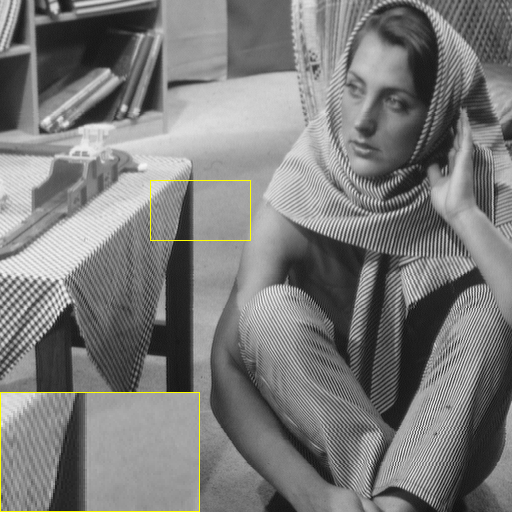
\includegraphics[width=0.2\linewidth]{4-5-1}
	}\hspace{-0.01\linewidth}
	\subfigure[fix 1/24.20]{
		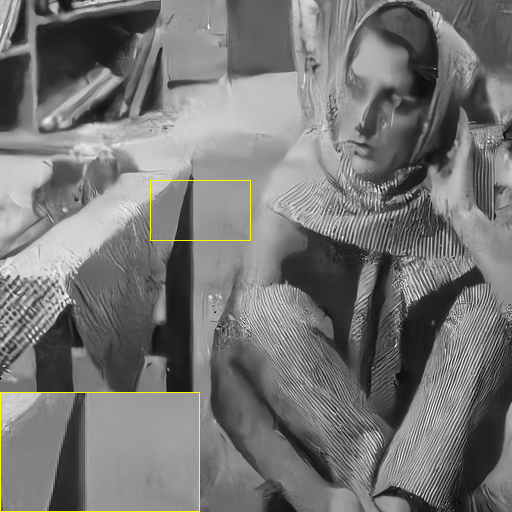
\includegraphics[width=0.2\linewidth]{4-5-3}
	}\hspace{-0.01\linewidth}
	\subfigure[B=1/26.64]{
		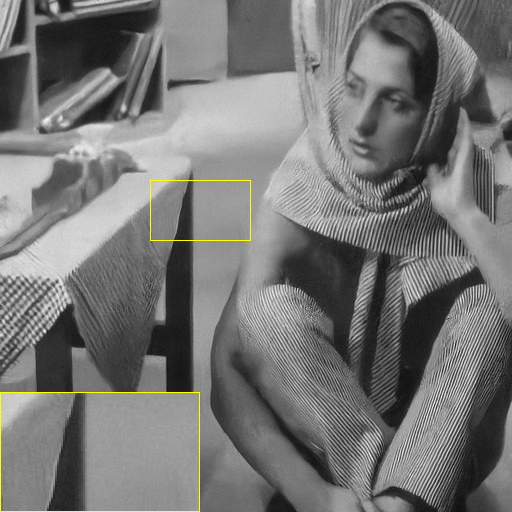
\includegraphics[width=0.2\linewidth]{4-5-5}
	}\hspace{-0.01\linewidth}
	\subfigure[fix 4/{\color{red}26.89}]{
		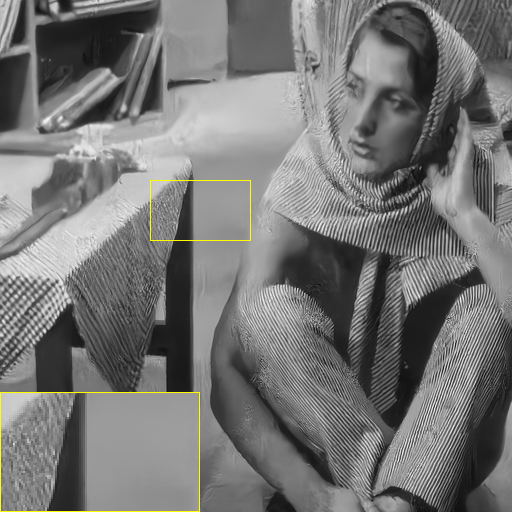
\includegraphics[width=0.2\linewidth]{4-5-7}
	}
	
	\subfigure[Original]{
		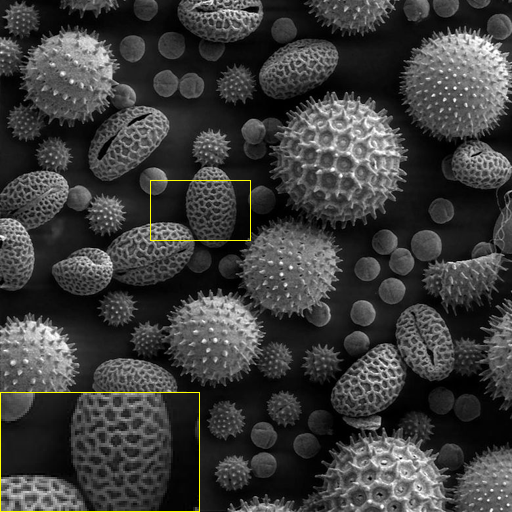
\includegraphics[width=0.2\linewidth]{4-5-2}
	}\hspace{-0.01\linewidth}
	\subfigure[fix 1/22.39]{
		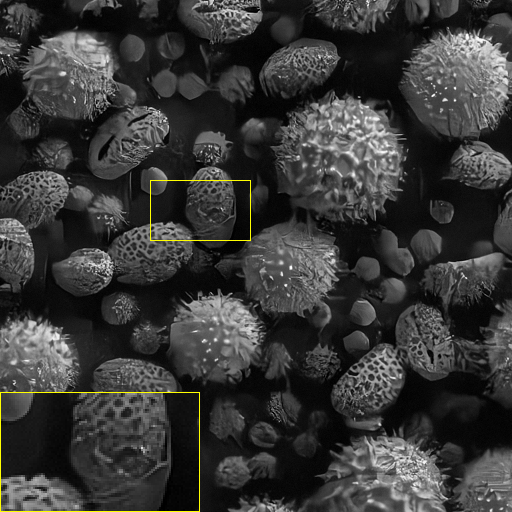
\includegraphics[width=0.2\linewidth]{4-5-4}
	}\hspace{-0.01\linewidth}
	\subfigure[B=1/25.49]{
		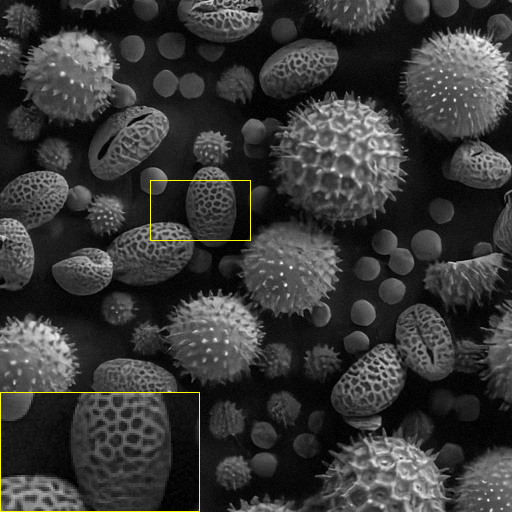
\includegraphics[width=0.2\linewidth]{4-5-6}
	}\hspace{-0.01\linewidth}
	\subfigure[fix 4/{\color{red}25.55}]{
		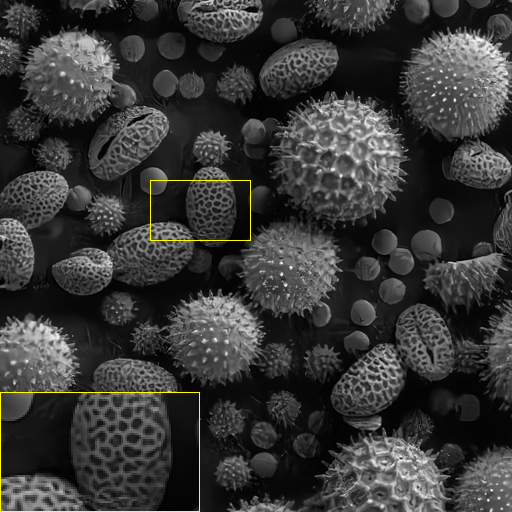
\includegraphics[width=0.2\linewidth]{4-5-8}
	}
	\caption{SOCE算法在DnCNN下不同mini-batch的重构结果}
	\label{fig:4-5} 
\end{figure}
\begin{figure}[!htbp]
	\centering
	\subfigure[Original]{
		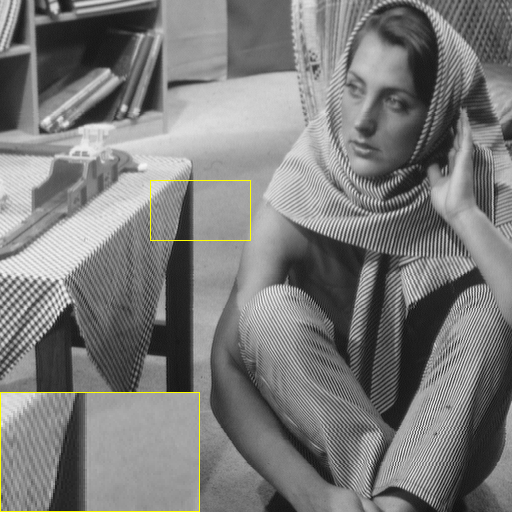
\includegraphics[width=0.2\linewidth]{4-6-1}
	}\hspace{-0.01\linewidth}
	\subfigure[fix 1/23.92]{
		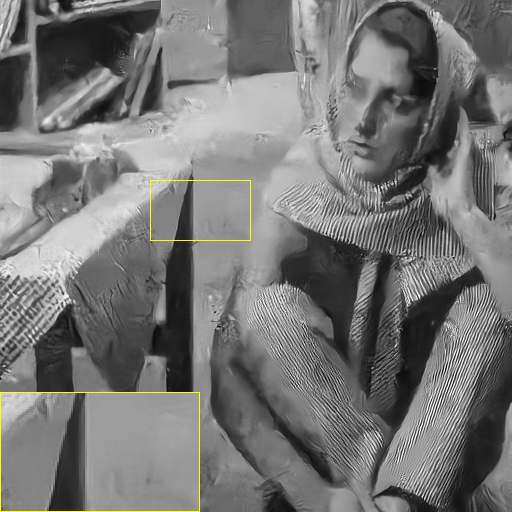
\includegraphics[width=0.2\linewidth]{4-6-3}
	}\hspace{-0.01\linewidth}
	\subfigure[B=1/26.42]{
		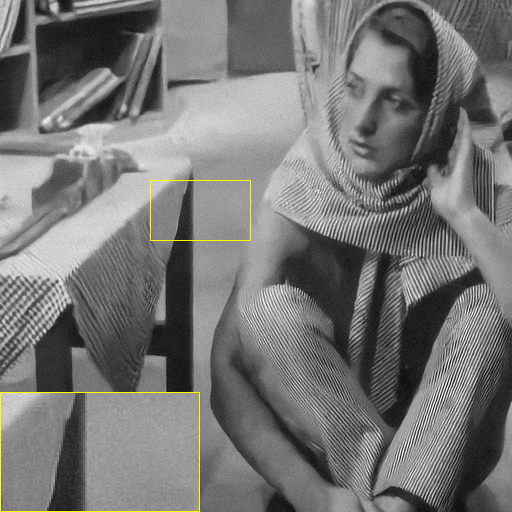
\includegraphics[width=0.2\linewidth]{4-6-5}
	}\hspace{-0.01\linewidth}
	\subfigure[fix 4/{\color{red}26.57}]{
		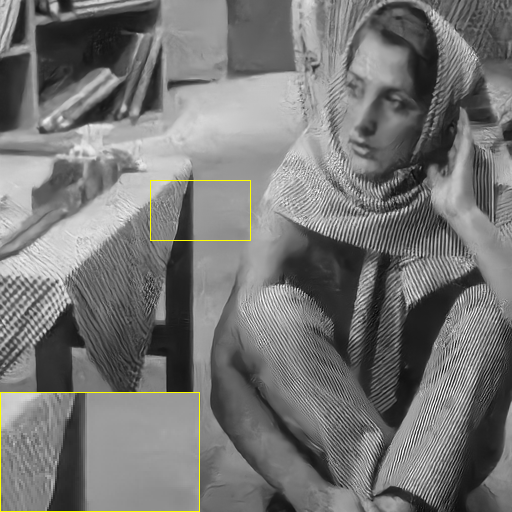
\includegraphics[width=0.2\linewidth]{4-6-7}
	}
	\\
	\subfigure[Original]{
		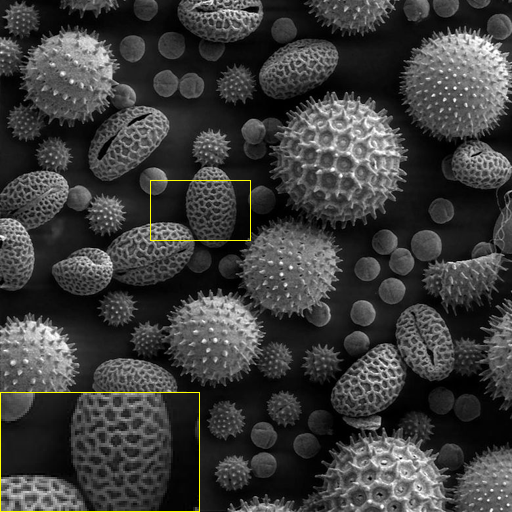
\includegraphics[width=0.2\linewidth]{4-6-2}
	}\hspace{-0.01\linewidth}
	\subfigure[fix 1/22.58]{
		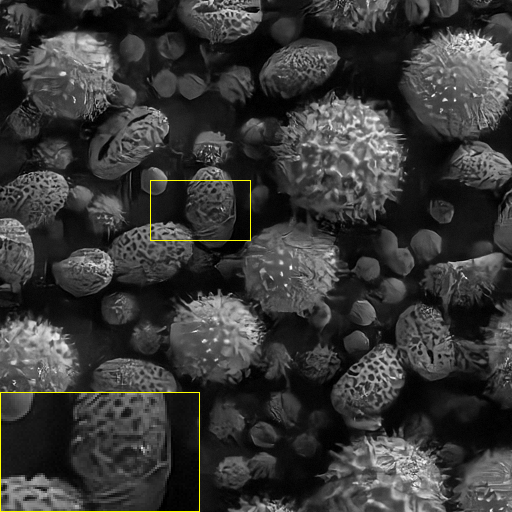
\includegraphics[width=0.2\linewidth]{4-6-4}
	}\hspace{-0.01\linewidth}
	\subfigure[B=1/25.09]{
		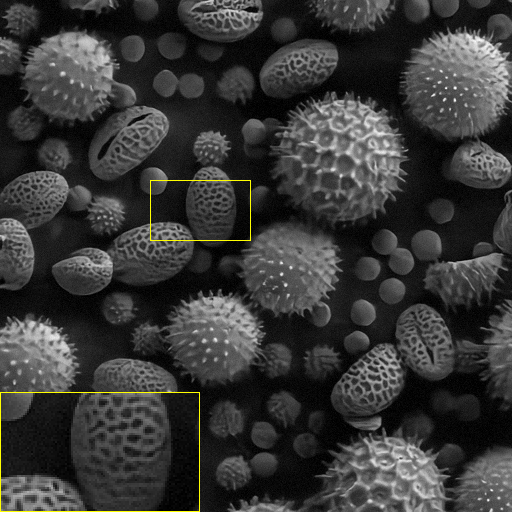
\includegraphics[width=0.2\linewidth]{4-6-6}
	}\hspace{-0.01\linewidth}
	\subfigure[fix 4/{\color{red}25.61}]{
		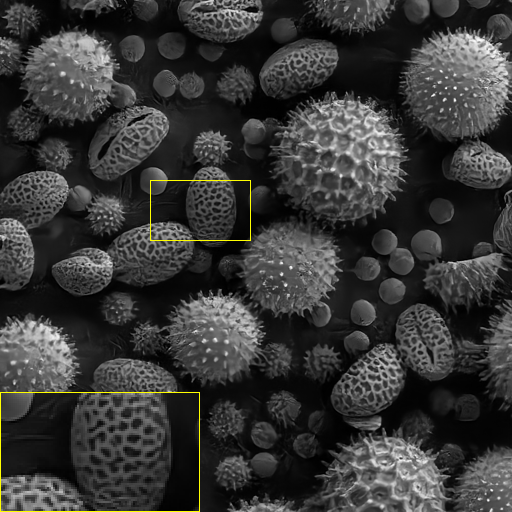
\includegraphics[width=0.2\linewidth]{4-6-8}
	}
	\caption{SOCE算法在IRCNN下不同mini-batch的重构结果}
	\label{fig:4-6}  
\end{figure}

为进一步验证SOCE算法的收敛性,本节给出了当去噪算子为IRCNN时,重构Barbara迭代过程中各个代理的利普希茨常数统计直方图,如图\ref{fig:4-7}所示。图\ref{fig:4-7}中的\subref{subfigure:4-2-1}为单个衍射图案时TACE算法数据保真项近邻算子与去噪器在迭代过程中的利普希茨常数统计直方图,\subref{subfigure:4-2-2}为$B=1$时SOCE算法数据保真项近邻算子与去噪器在迭代过程中的利普希茨常数统计直方图,\subref{subfigure:4-2-3}为四个衍射图案时TACE算法数据保真项近邻算子与去噪器在迭代过程中的利普希茨常数统计直方图。上层代表数据保真项的近邻算子,下层代表IRCNN去噪算子。在抗泊松噪声模型下,根据图\ref{fig:4-7}得出的SOCE算法收敛性结论与上节图\ref{fig:4-5}相同。
\begin{figure}[!htbp]
	\centering
	\subfigure[fix 1]{
		\label{subfigure:4-2-1}
		\begin{minipage}[t]{0.2\linewidth}
			\centering
			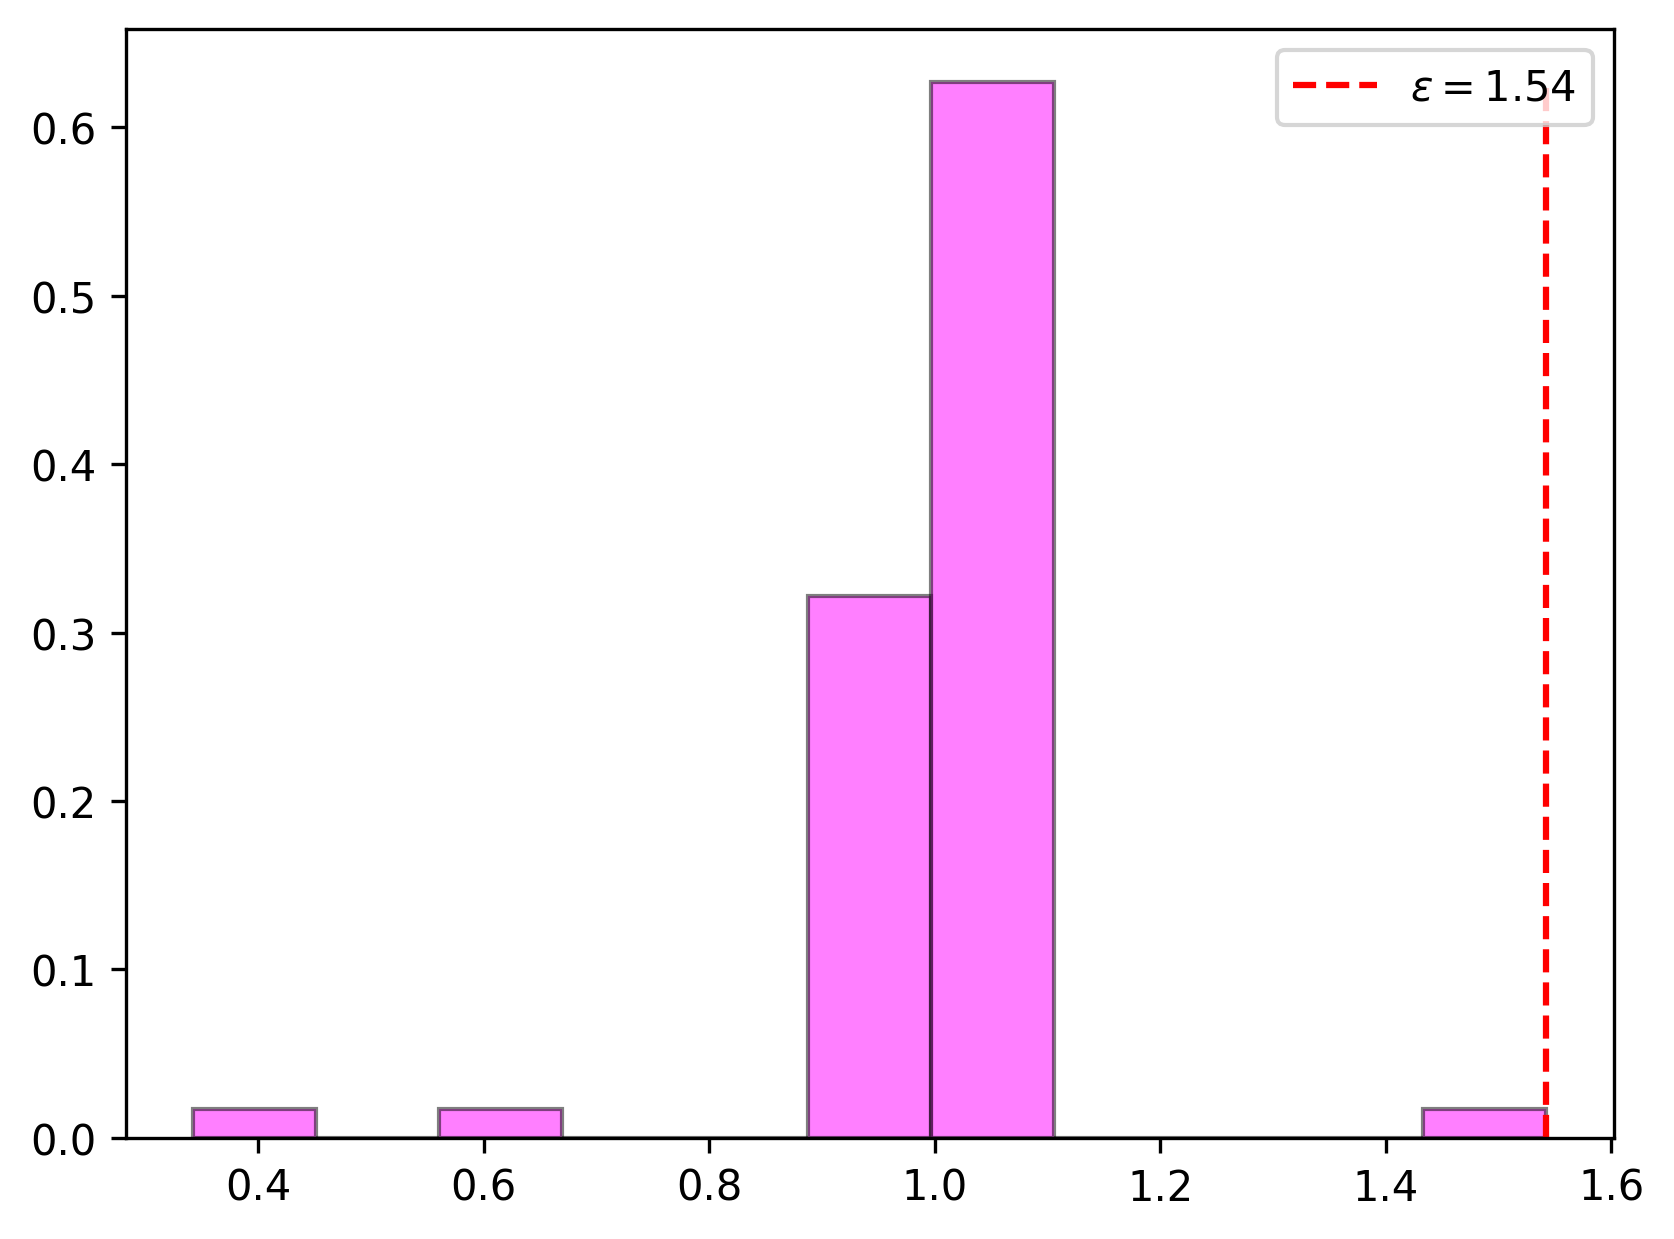
\includegraphics[width=\linewidth]{4-7-1}\\
			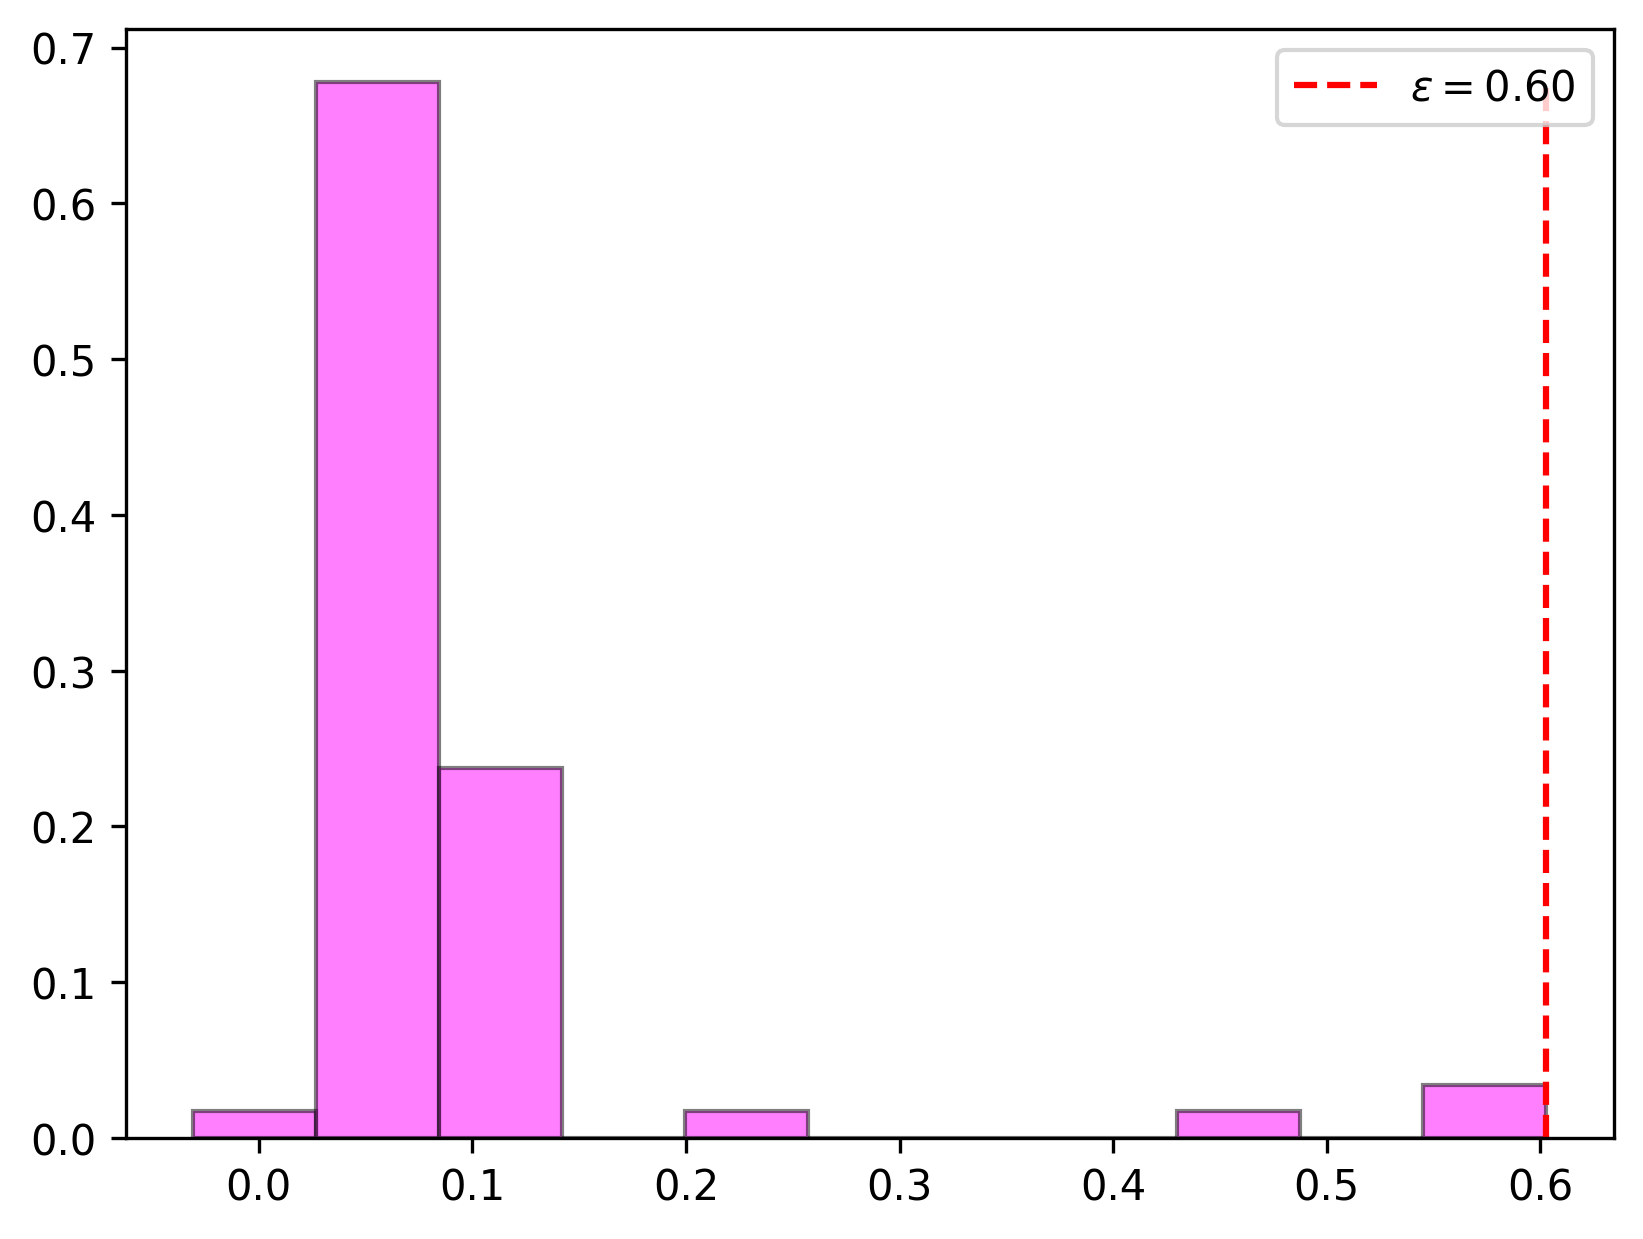
\includegraphics[width=\linewidth]{4-7-2}
			%\caption{fig}
		\end{minipage}
	}
	\subfigure[B=1]{
		\label{subfigure:4-2-2}
		\begin{minipage}[t]{0.2\linewidth}
			\centering
			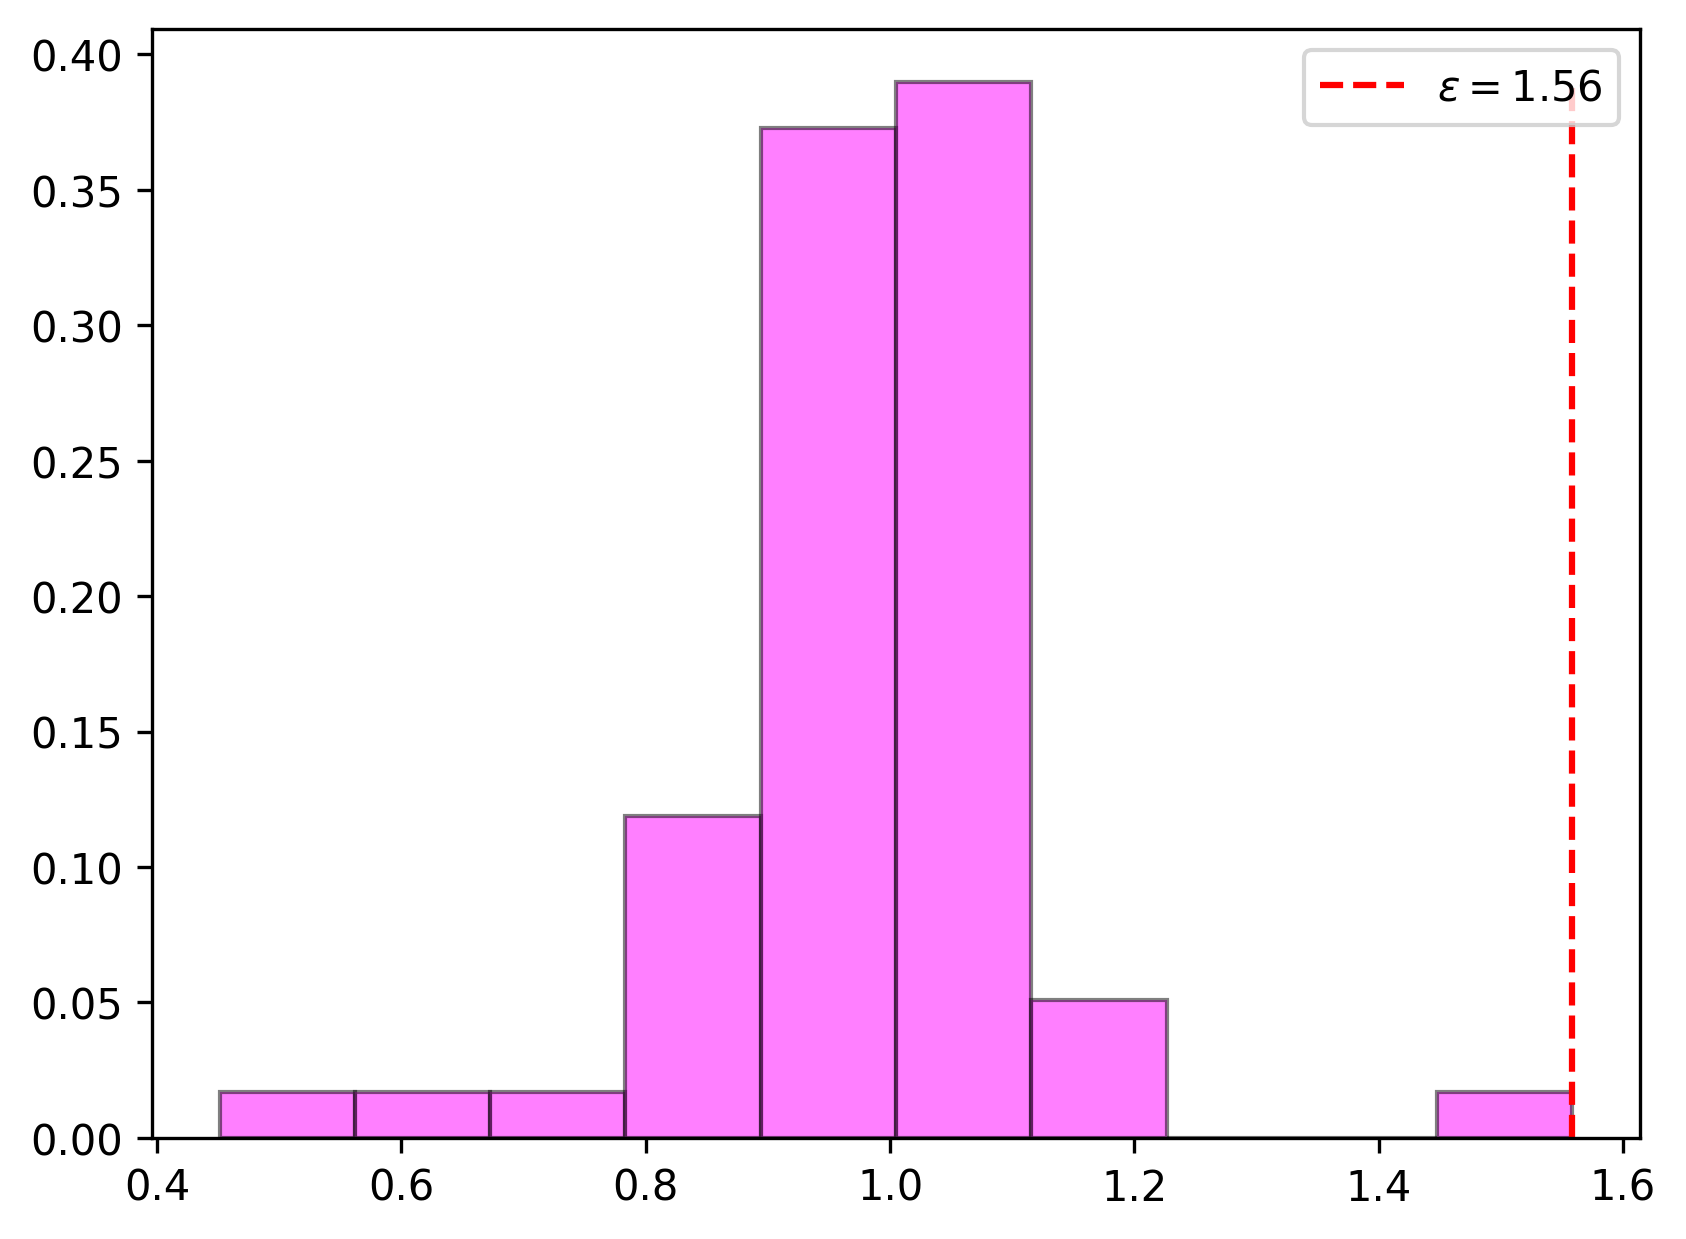
\includegraphics[width=\linewidth]{4-7-3}\\
			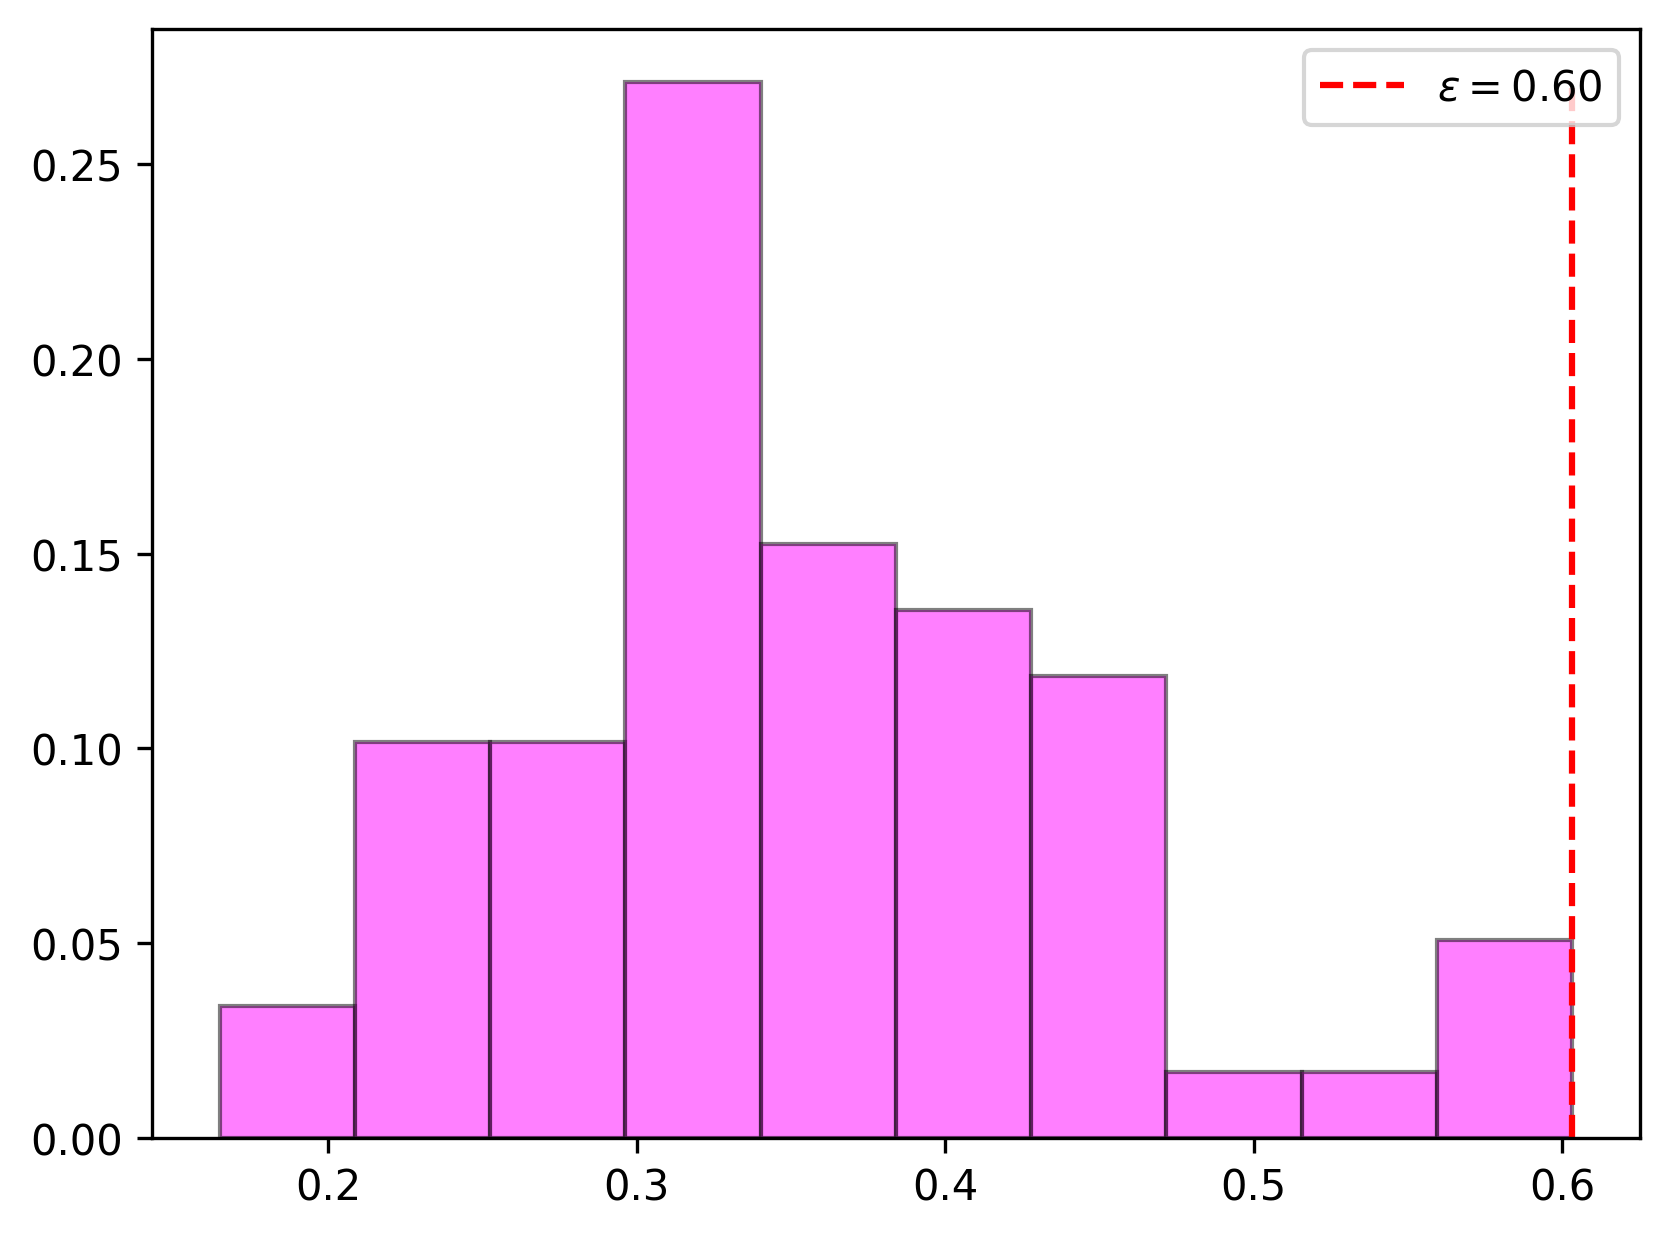
\includegraphics[width=\linewidth]{4-7-4}
			%\caption{fig}
		\end{minipage}
	}
	\subfigure[fix 4]{
		\label{subfigure:4-2-3}
		\begin{minipage}[t]{0.2\linewidth}
			\centering
			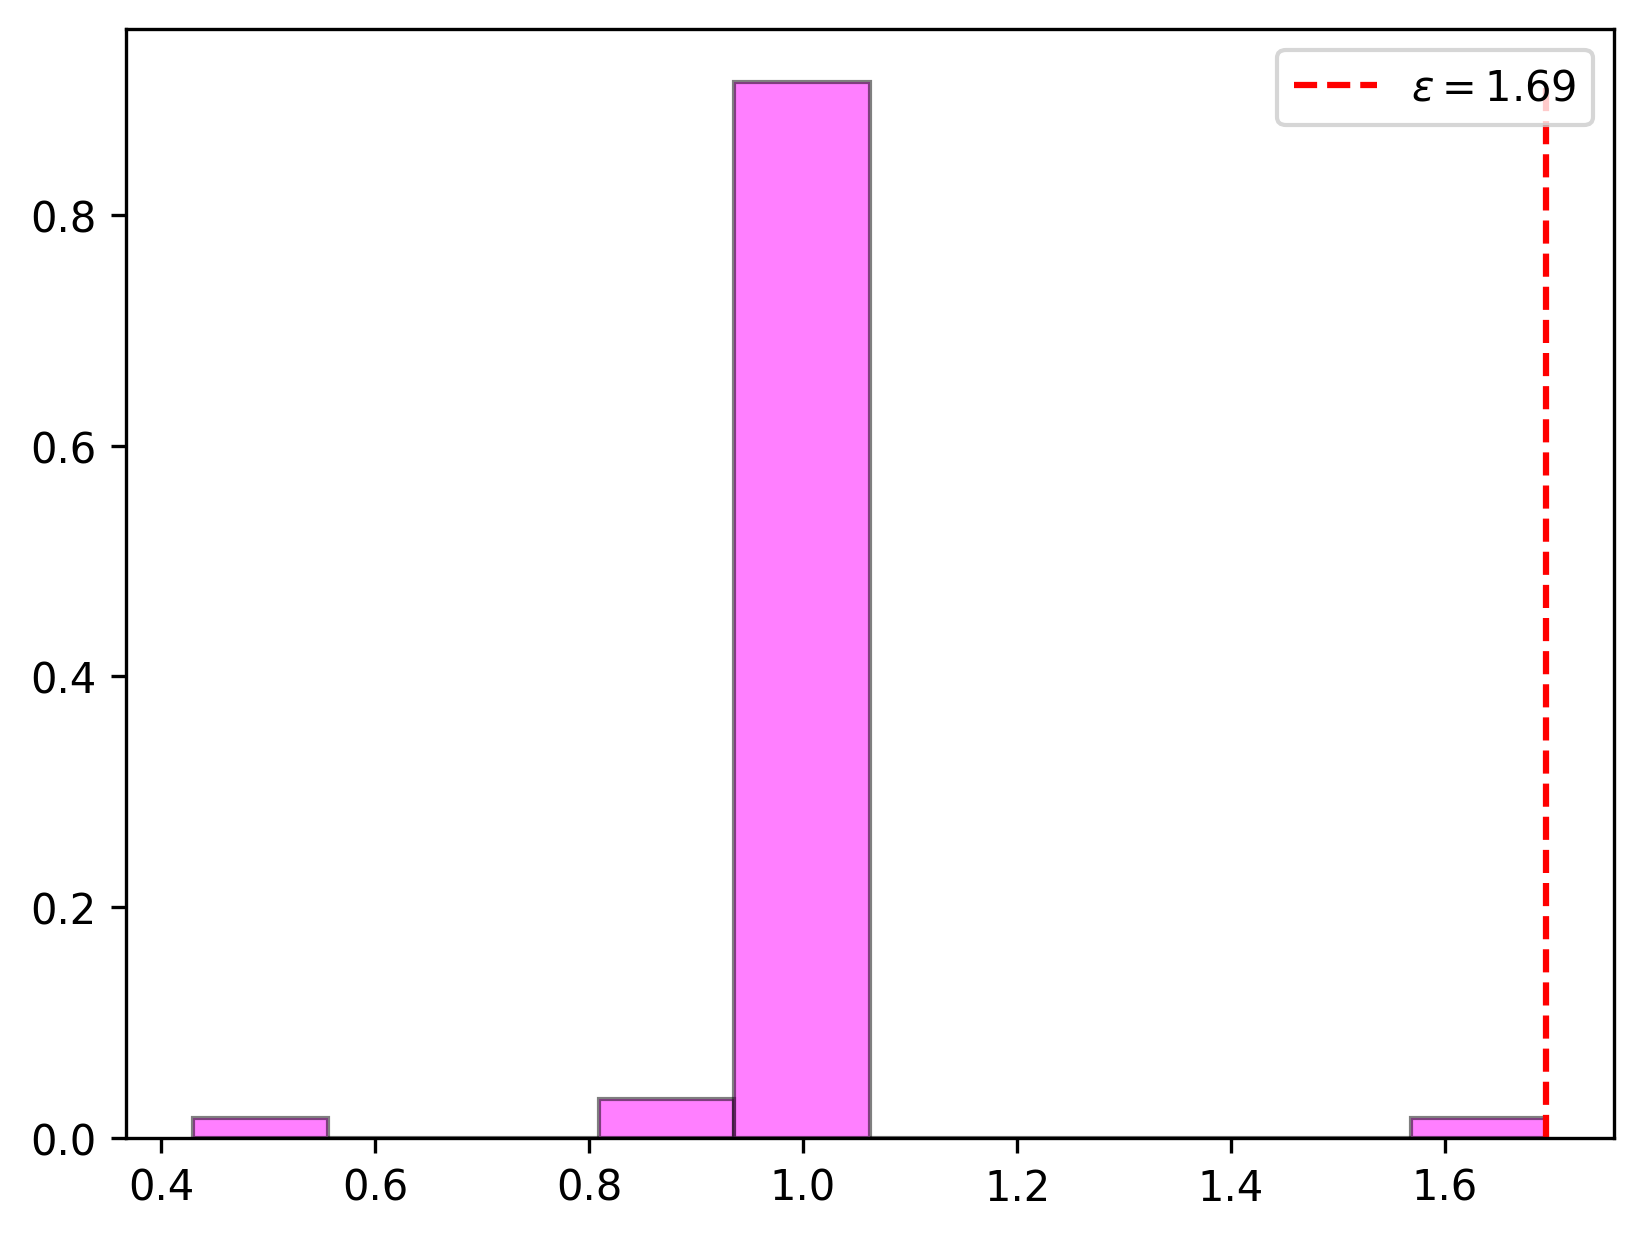
\includegraphics[width=\linewidth]{4-7-5}\\
			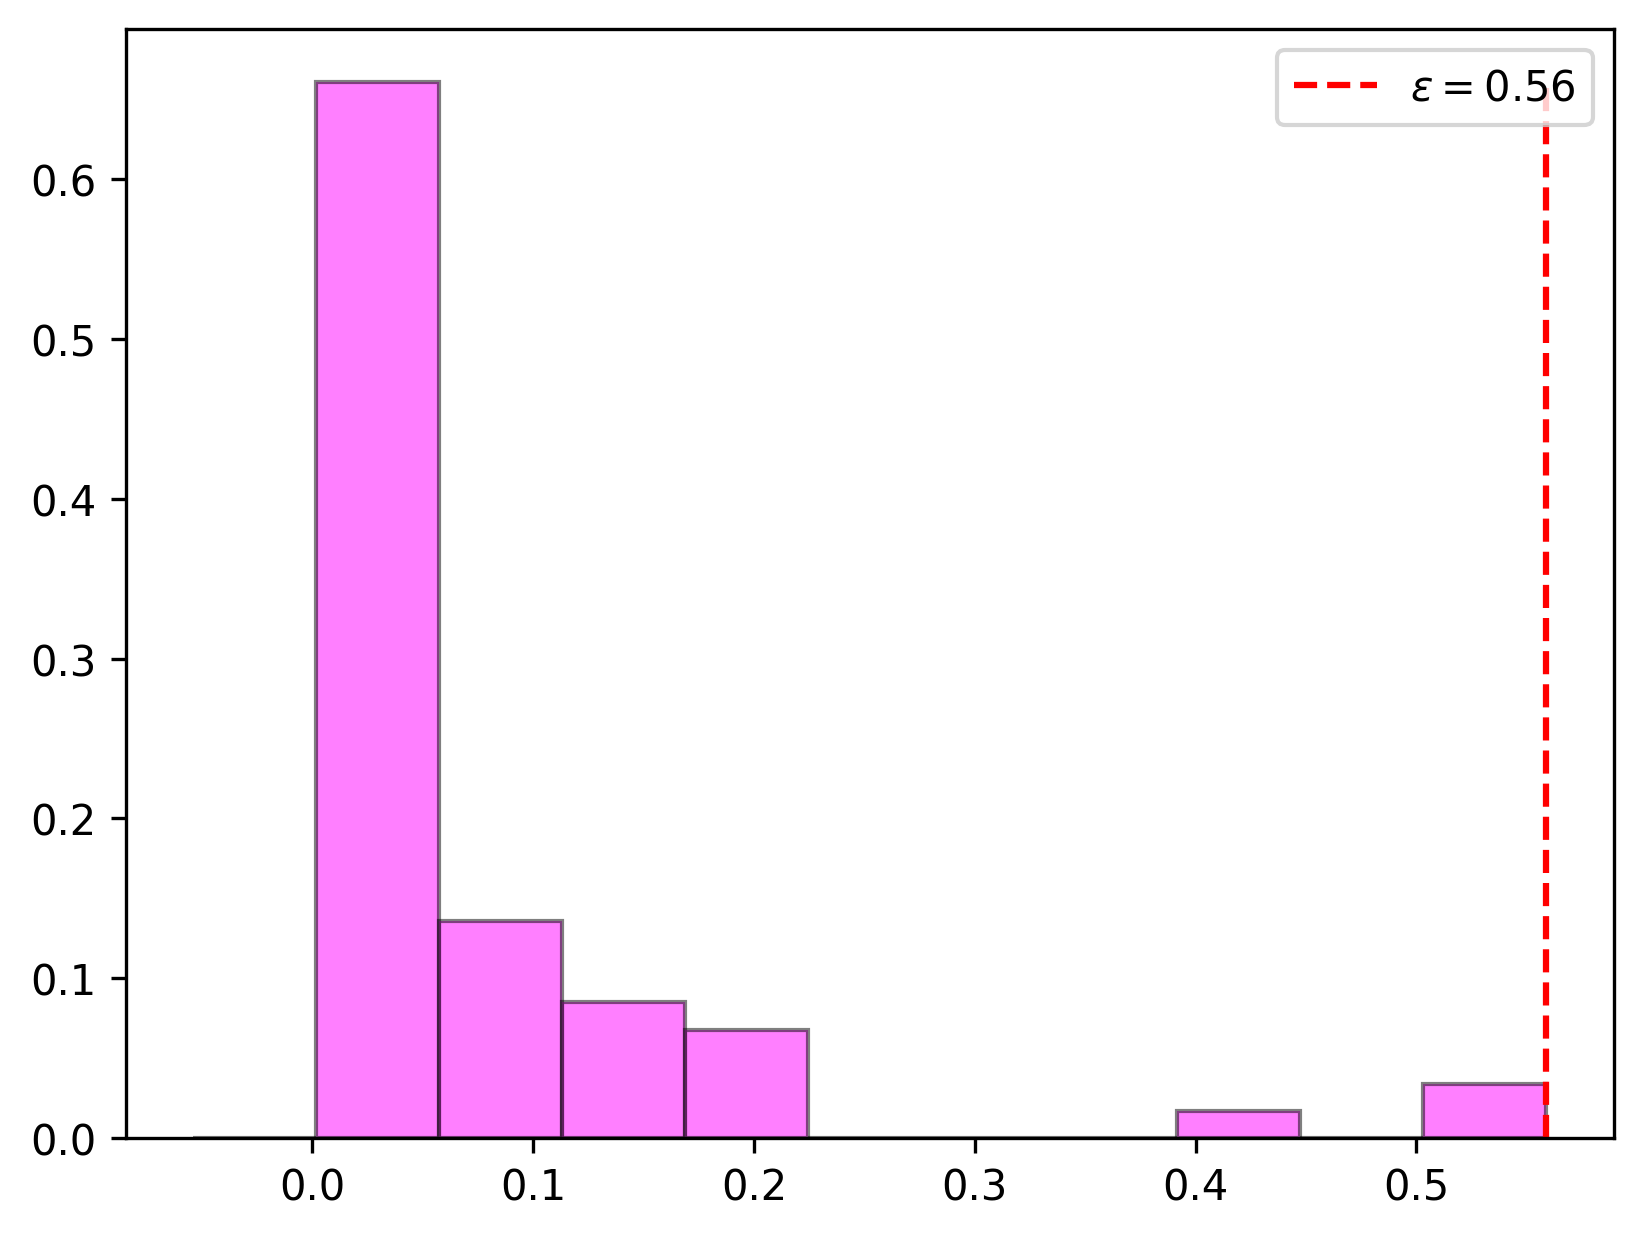
\includegraphics[width=\linewidth]{4-7-6}
			%\caption{fig}
		\end{minipage}
	}
	\caption{SOCE算法在迭代过程中的利普希茨常数统计直方图(IRCNN)} 
	\label{fig:4-7}  
\end{figure}

\section{本章小结}
首先分析了一阶随机优化算法的基本特性,然后提出了基于一阶随机优化的编码衍射成像法,并通过大量实验证明了该算法的有效性。实验结果表明了在编码衍射模型下,该算法可看作为TACE算法的加速版本,对处理大规模编码衍射图案有着较大的优势。